\chapter{The role of vertical structure in QBO teleconnections}
\label{cha:deepQBO}

\section{Introduction}
\label{sec:deepQBO-introduction}

Findings from chapter 3 indicated an association between a vertically integrated QBO index and the vortex. While a large body of work has aimed to understand teleconnections between the equatorial winds and the vortex (see section \ref{sec:external_influence_HT}), aspects of the connection between the QBO and other parts of the stratosphere as well as the troposphere and surface, evade definitive explanation.

The QBO is typically defined by the equatorial ZMZW at a single level in the mid-stratosphere. The 50 hPa level is usually used for observational studies into teleconnections between the QBO and NH variability \citep{Baldwin2001, Baldwin98}. However, some studies have also noted the importance of characterising the vertical structure of the QBO \citep{Fraedrih1993, Wallace1993,  Baldwin98,  Dunkerton2017, graySurface2018, andrewsObserved2019}. In an observational-based study \cite{graySurface2018} find an enhanced association between the QBO and polar vortex as well as MSLP anomalies over the NH when a metric incorporating the vertical coherence of equatorial winds via empirical orthogonal functions is utilised (such an EOF method is first presented in \citep{verena2016a}). The same work proposes three distinct physical pathways by which the QBO exerts influence over tropospheric and surface variations: via modulation of NH winter vortex strength (the HT effect), through influence over tropical upwelling brought about by the induced meridional circulation associated with different QBO phases (ref) and finally via alterations in horizontal temperature gradients in the tropospheric subtropical jet region also caused by the induced meridional circulation. The same work shows that the nature of responses in the vortex and surface to the QBO vary significantly within the NH winter season with midwinter responses (in January) sensitive to QBO winds near 50hPa in contrast to early and later winter (February and March) responses which are most sensitive to the QBO defined at 20hPa and 70hPa. In a subsequent model-based study \cite{andrewsObserved2019} introduce a similar but simpler methodology by defining the QBO as the average ZMZW between two vertical levels, which preferentially selects time intervals that display a vertically coherent QBO phase between the specified levels. The same study reports enhanced responses to the QBO from the NAO and Arctic Oscillation (AO) when such vertically integrated metrics are used to define QBO phase compared to a single level definition. 

In addition to the QBO, variations in ZMZW in the upper stratosphere and lower mesosphere, the SAM (see section \ref{sec:equatorial_strat}), also shows associations with the vortex. The influence of the SAO on vortex variability and SSWs was first hypothesised in the observational study of \cite{JGray2001} which used rocketsonde data to establish a link between the vertical extent of the westerly SAO phase and vortex strength. However these results statistically significant and the work stressed the need for more study with comprehensive observations as well as model simulations. Subsequent studies found similar links but with varying features. \cite{Gray2003} found influence of upper stratosphere equatorial winds and SSWs over the whole season but mostly in mid winter. This was attributed to timing of the phase transition from westerly to easterly SAO. \cite{JGray2001} and \cite{Hamilton} suggest that equatorial winds at all stratospheric levels (including the QBO and SAO regions) influence the vortex and a combination of QBO and SAO conditions is required to obtain a significant signal in vortex variability.

While many studies highlight statistical associations between QBO metrics as well as the SAO with other parts of the climate system, they are less effective at demonstrating causal relationships. Indeed, \cite{andrewsObserved2019} note the possibility that both the occurrence of deep QBO phases and NAO and AO anomalies may be driven by an unidentified third factor which may give rise to a robust statistical link between the phenomena without any direct physical connection. Some studies aim to overcome this potential pitfall and explicitly test the natures of dynamical features with forced model setups, where momentum forcing or nudging is applied to winds in specific regions of the atmosphere. Such works further suggest the importance of the SAO and QBO region when considering the vortex. \cite{Pascoe2005} finds improved vortex representation in model runs with forced winds in the equatorial stratosphere (both QBO and SAO regions separately) and \cite{Brown2019} shows that nudging model winds in the SAO region (as well as specifying tropospheric wave forcing) towards reanalysis for a single winter, allows the model to capture an SSW observed in that winter with high degrees of accuracy in its timing and magnitude.   

Despite the significant body of work presented above into the QBO and its relation to other parts of the climate system, the role of vertical structure in teleconnections is not fully understood. In this chapter, we utilise a set of nudging experiments to explicitly test the importance of vertical coherence in the equatorial stratosphere's influence over the vortex as well as tropospheric and surface variability. Results form this analysis may aid in establishing the true nature of QBO teleconnections as well as develop understanding of a potentially powerful source of forecast predictive skill (the equatorial stratosphere).

\section{Model Configuration}

To explicitly test the effect of QBO vertical coherence on teleconnections we utilise a set of custom designed simulations which utilises a modified version of the UKESM GCM analysed in chapters 3 and 4. As with the pi-control simulation examined so far, the model component for the atmosphere is GA7.1, GHG concentrations are set to 1850 levels (see section \ref{sec:model_config}) and volcanic eruptions are absent (however a constant background volcanic aerosol level is imposed). The primary difference between the pi-control and the configuration utilised here is the experiments run with no coupled Ocean component. Instead, SSTs are prescribed using a seasonally invariant climatological field obtained from an interval of the the pi-control (year numbers 96-126). Sea Ice extents are also prescribed to climatological values using the same interval of the pi-control and full documentation for this type of timeslice experiment is provided in \cite{oconnorAssessment2021}. All simulations are initialised using conditions from the start of the 30 year interval of the pi-control used to calculate SST and SI climatologies (year number 96). We choose to impose SST and sea ice conditions in our experiments as this removes contributions to atmospheric circulation from interannual to decadal surface modes of variability such as ENSO and the AL. This in turn isolates the effect of the QBO further as any differences in QBO-vortex and QBO-surface interactions across the simulations are not due to coupling with SSTs and other surface boundary conditions.  %Analysis chapters 4 and 5 showed that this year does not lie in an interval in which the QBO or the vortex exhibits significant multi-decadal oscillations. As a result, the initial conditions for the simulation are less likely samples the QBO and vortex in a randomly chosen state.

\subsection{Nudging}
In order to impose the vertical structure of the QBO in our sensitivity experiments we employ a method to constrain atmospheric conditions in a GCM simulation known as nudging. In this method, an atmospheric quantity, $Y$, is constrained via Newtonian-relaxation which pushes the model state for $Y$ towards some imposed value at each model timestep such that

\begin{equation} \label{eq:nudging}
\Delta Y = G \Delta t (Y_{imposed} - Y_{model}), 
\end{equation}

where $Y_{imposed}$ is the state of $Y$ from the imposed field, $Y_{model}$ is the value of $Y$ the model has evolved to since the last timestep (when it was last nudged), $\Delta Y$ is the change in $Y$ applied by the nudging scheme and $G$ is the relaxation parameter. $G$ is a measure of the strength of the relaxation towards $Y_{imposed}$ at each timestep and can also be expressed as $G = \frac{1}{\tau}$ where $\tau$ is known as the relaxation timescale. When choosing the relaxation timescale, a balance is required between constraining the model sufficiently to the imposed state (I.E. a short enough $\tau$ such that the model's $Y$ avoids evolving freely) and avoiding the introduction of large gradients (a large enough $\tau$ to avoid model instability). The MetOffice Unified model, of which the model configurations presented here are a part, typically uses a relaxation timescale of 6 hours at all vertical levels. This has been shown to produce good quality nudging results in a range of studies employing such a method despite the different radiative timescales present across atmospheric levels (Brown et al. 2020). In our experiments we to nudge the zonal wind, $U$, towards an idealised version of the QBO wind fields expressed as 

\begin{equation} \label{eq:imposed_U}
U_{qbo}(t, z) = F(z) sin(\frac{2\pi (t + zs)}{period}),
\end{equation}

Where $s$ is a parameter which sets the rate of phase shift with descending height. We set $s$ to xxxx and the For the deep QBO experiment (that which displays a high degree of vertical coherence) and xxx for the shallow QBO to ensure a large phase shift with height (and therefore less vertical coherence). We choose the period of the QBO in both experiments to be xxx months for consistency with the QBO period exhibited in the UKESM pi-control. $F(z)$ is a momentum forcing vertical profile (seen in figure xxx) applied to reproduce the variation in magnitude of the QBO with height. Following the methodology of Pascoe et al., we use an $F(z)$ which takes the form of a Weibull function given by

\begin{equation} \label{eq:vertical_profile}
F(z) = R_D \frac{1}{\gamma \beta^\alpha}  Z_D^{\alpha-1}  e^{-Z_D/\beta},
\end{equation}

where the parameters are set to $\alpha = 3.5, \beta = 0.27, \gamma = 3.2335, R_D = 40.0 ms^{-1}, Z_{D} = (z - 15)/20$. The idealised time-height QBO profiles generated for both experiments are shown in figure xxxxa, they highlight the differences between idealised QBOs: The deep QBO winds exhibits the same sign of wind throughout the middle atmosphere for the majority of the series while the shallow QBO show different phases between the upper and middle stratosphere. In both experiments we apply the relaxation in equation \ref{eq:nudging} towards the corresponding QBO winds over the set of atmospheric levels approximately corresponding to the pressure level range xx-xxhPa and the latitudinal range xx-xx. The relaxation is applied at all longitudes. At the boundary between of these ranges we apply a tapered version of the relaxation with a value of that parameter $G$ that decreases linearly with increased distance from the relaxation region. This tapering is applied on the 2 atmospheric levels at the bottom and top of the vertical region and 5$^\circ$ either side of the latitudinal region. This tapering is applied to avoid introducing large vertical and latitudinal gradients in zonal wind and prevent potential model instability. 

\begin{figure}[h!]
\begin{center}
\noindent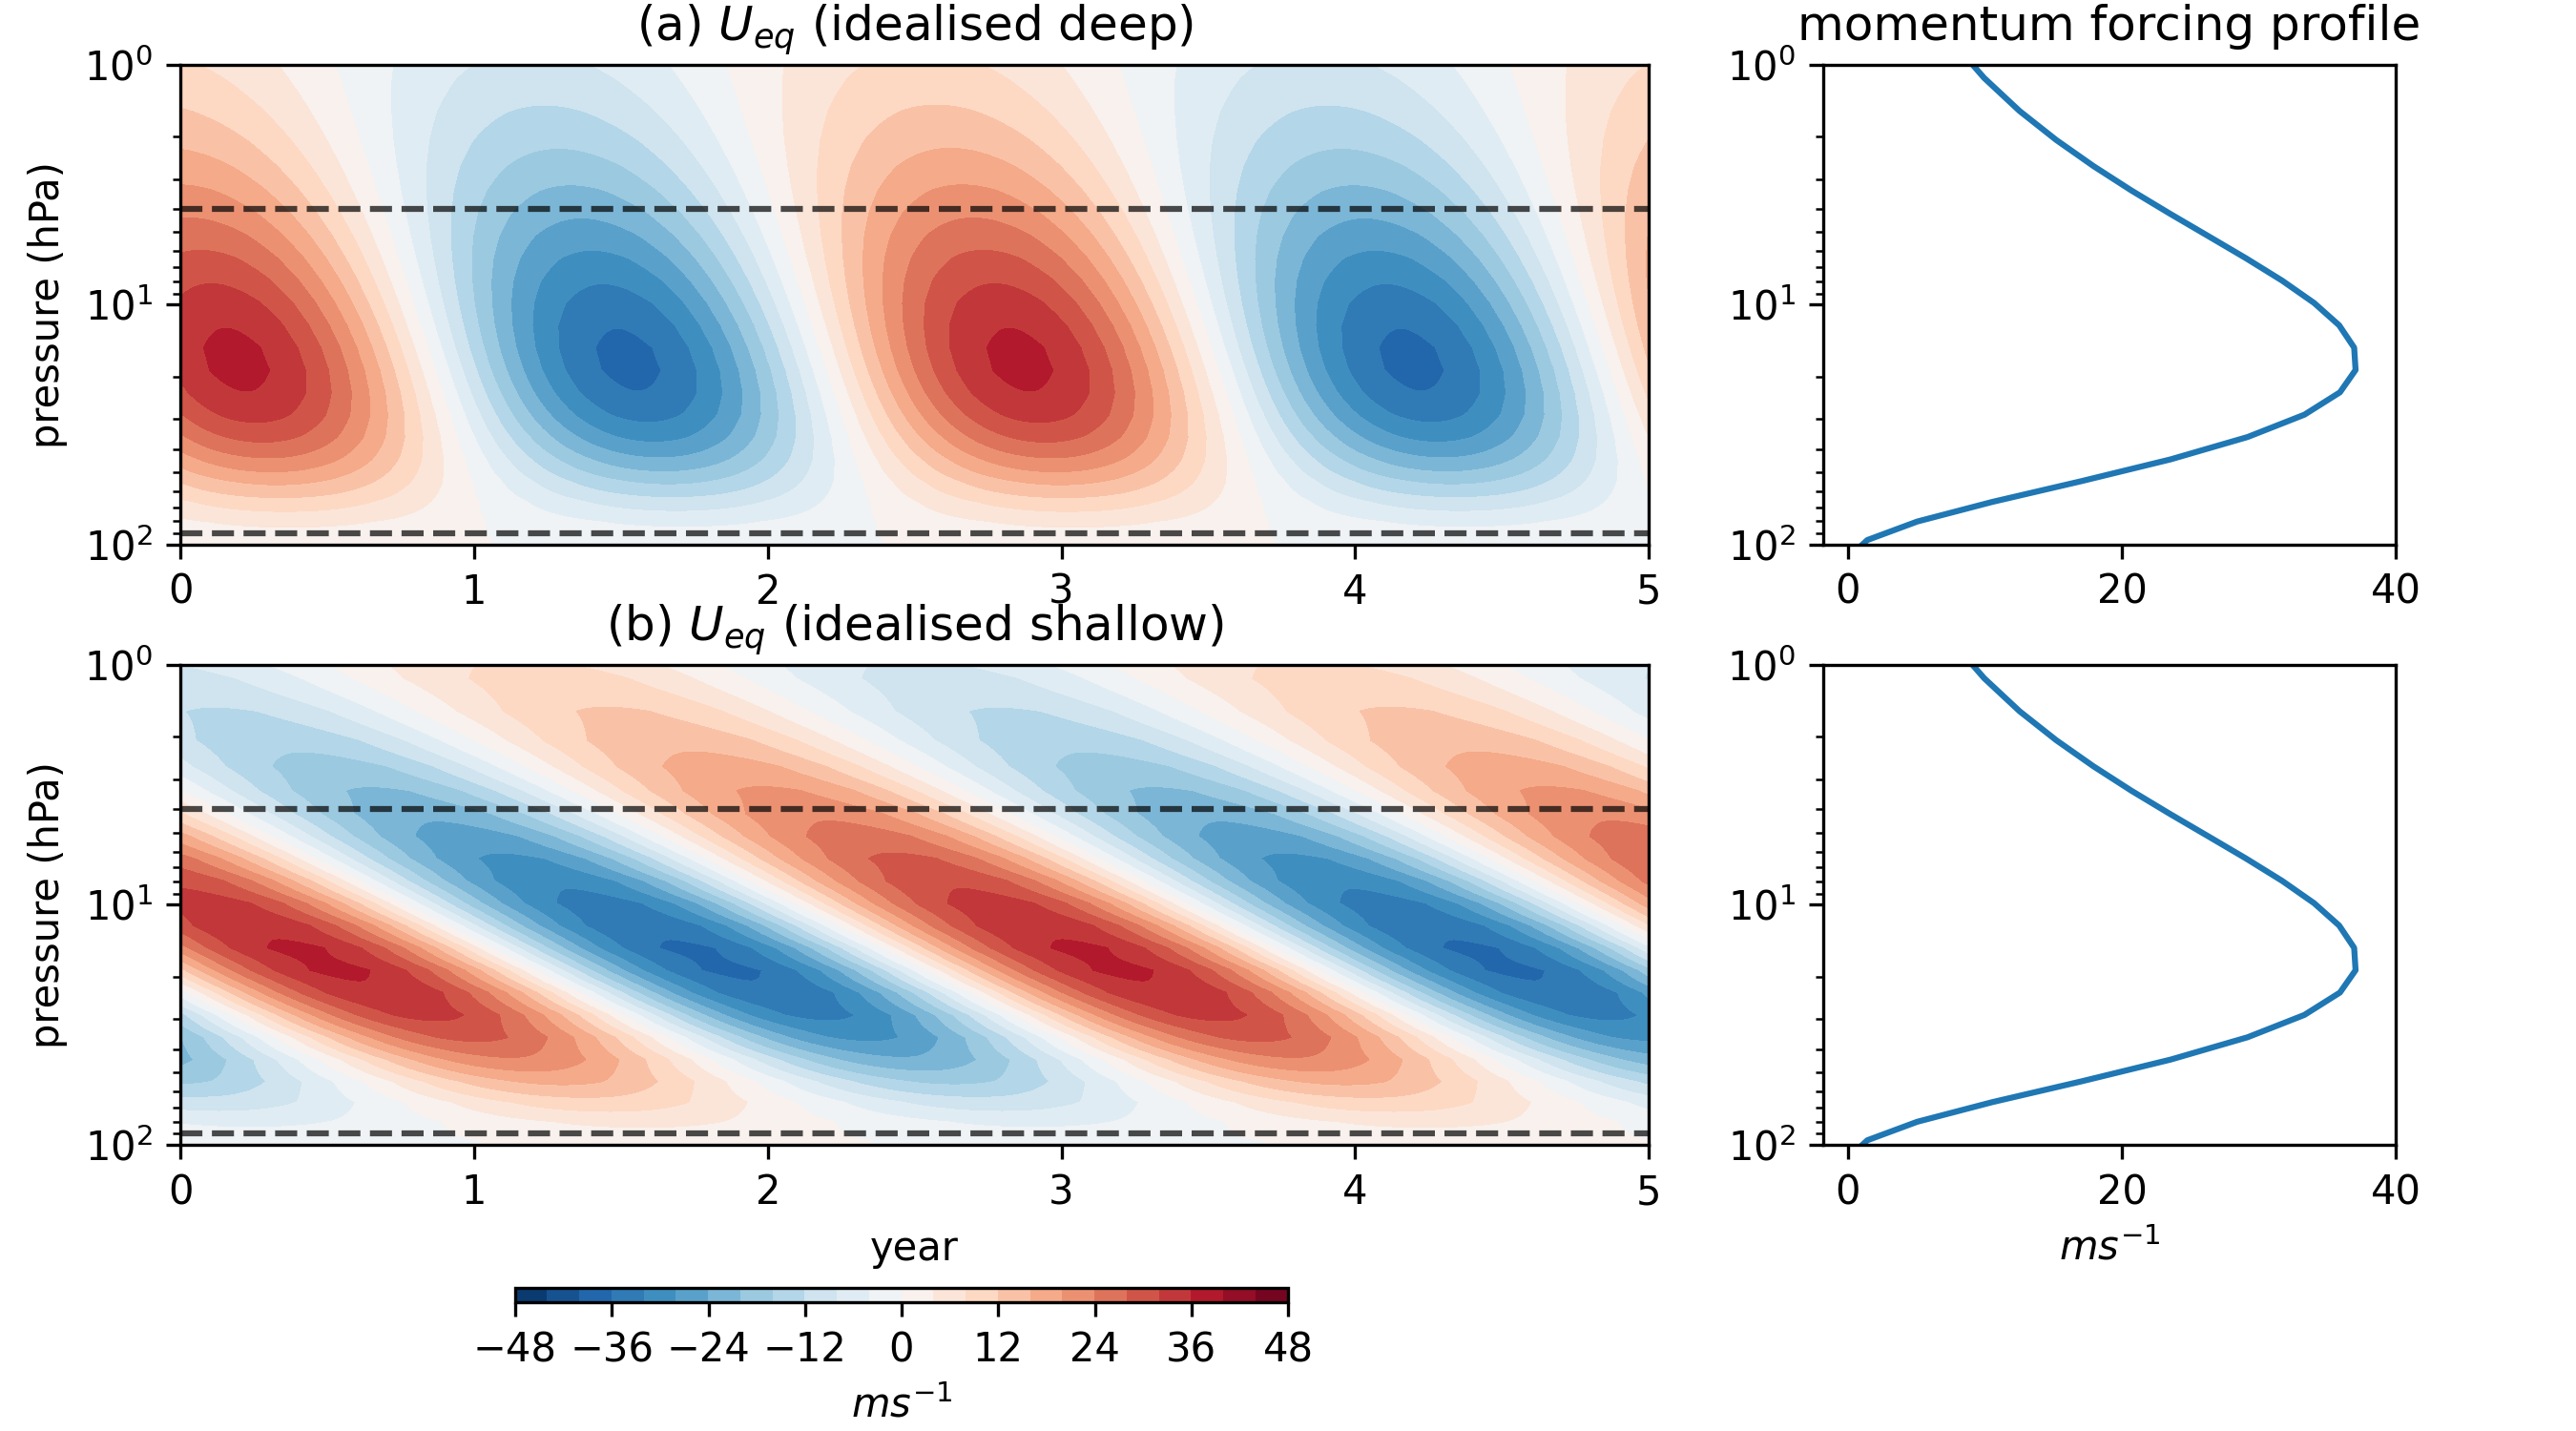
\includegraphics[width = \linewidth]{Figures/Figures-deepQBO/Idealised_QBO_features.png}
\caption[Idealised QBO winds used for nudging experiments]{Sample time-series of idealised equatorial ZMZW and associated momentum forcing profile for the deep (\textbf{a} and \text{b} respectively) and shallow (\textbf{c} and \textbf{d} respectively) QBO experiments. Horizontal dashed lines on (a) and (c) denote the xxhPa and 90hPa pressure levels between which we implement nudging towards the idealised wind in each experiment.}
\label{fig:Idealised_QBO_samples}
\end{center}
\end{figure}


\section{QBO Characteristics}
We first analyse the equatorial winds in each experiment and verify whether the implementation of nudging has resulted in the desired equatorial ZMZW profiles. Figure \ref{fig:experiment_QBOs}a and c show a 5 year sample of the the equatorial winds in each experiment that results from implementing QBO nudging between the 90hPa and 5hPa levels. These winds reflect many of the key features of the idealised winds (figure \ref{fig:Idealised_QBO_samples}a and c) - the deep experiment exhibits vertical coherence in the middle stratosphere while the shallow simulation shows opposite phases of the QBO in the upper and lower stratosphere. The period of ZMZW variations in both experiments is indicated by the Fourier power spectra shown in figures \ref{fig:experiment_QBOs}b and d. The mid-stratospheric winds (90-$\sim$ 10hPa) exhibits peak Fourier power corresponding to a period close to the value specified by the idealised winds (32 months) in both experiments. 

\begin{figure}[h!]
\begin{center}
\noindent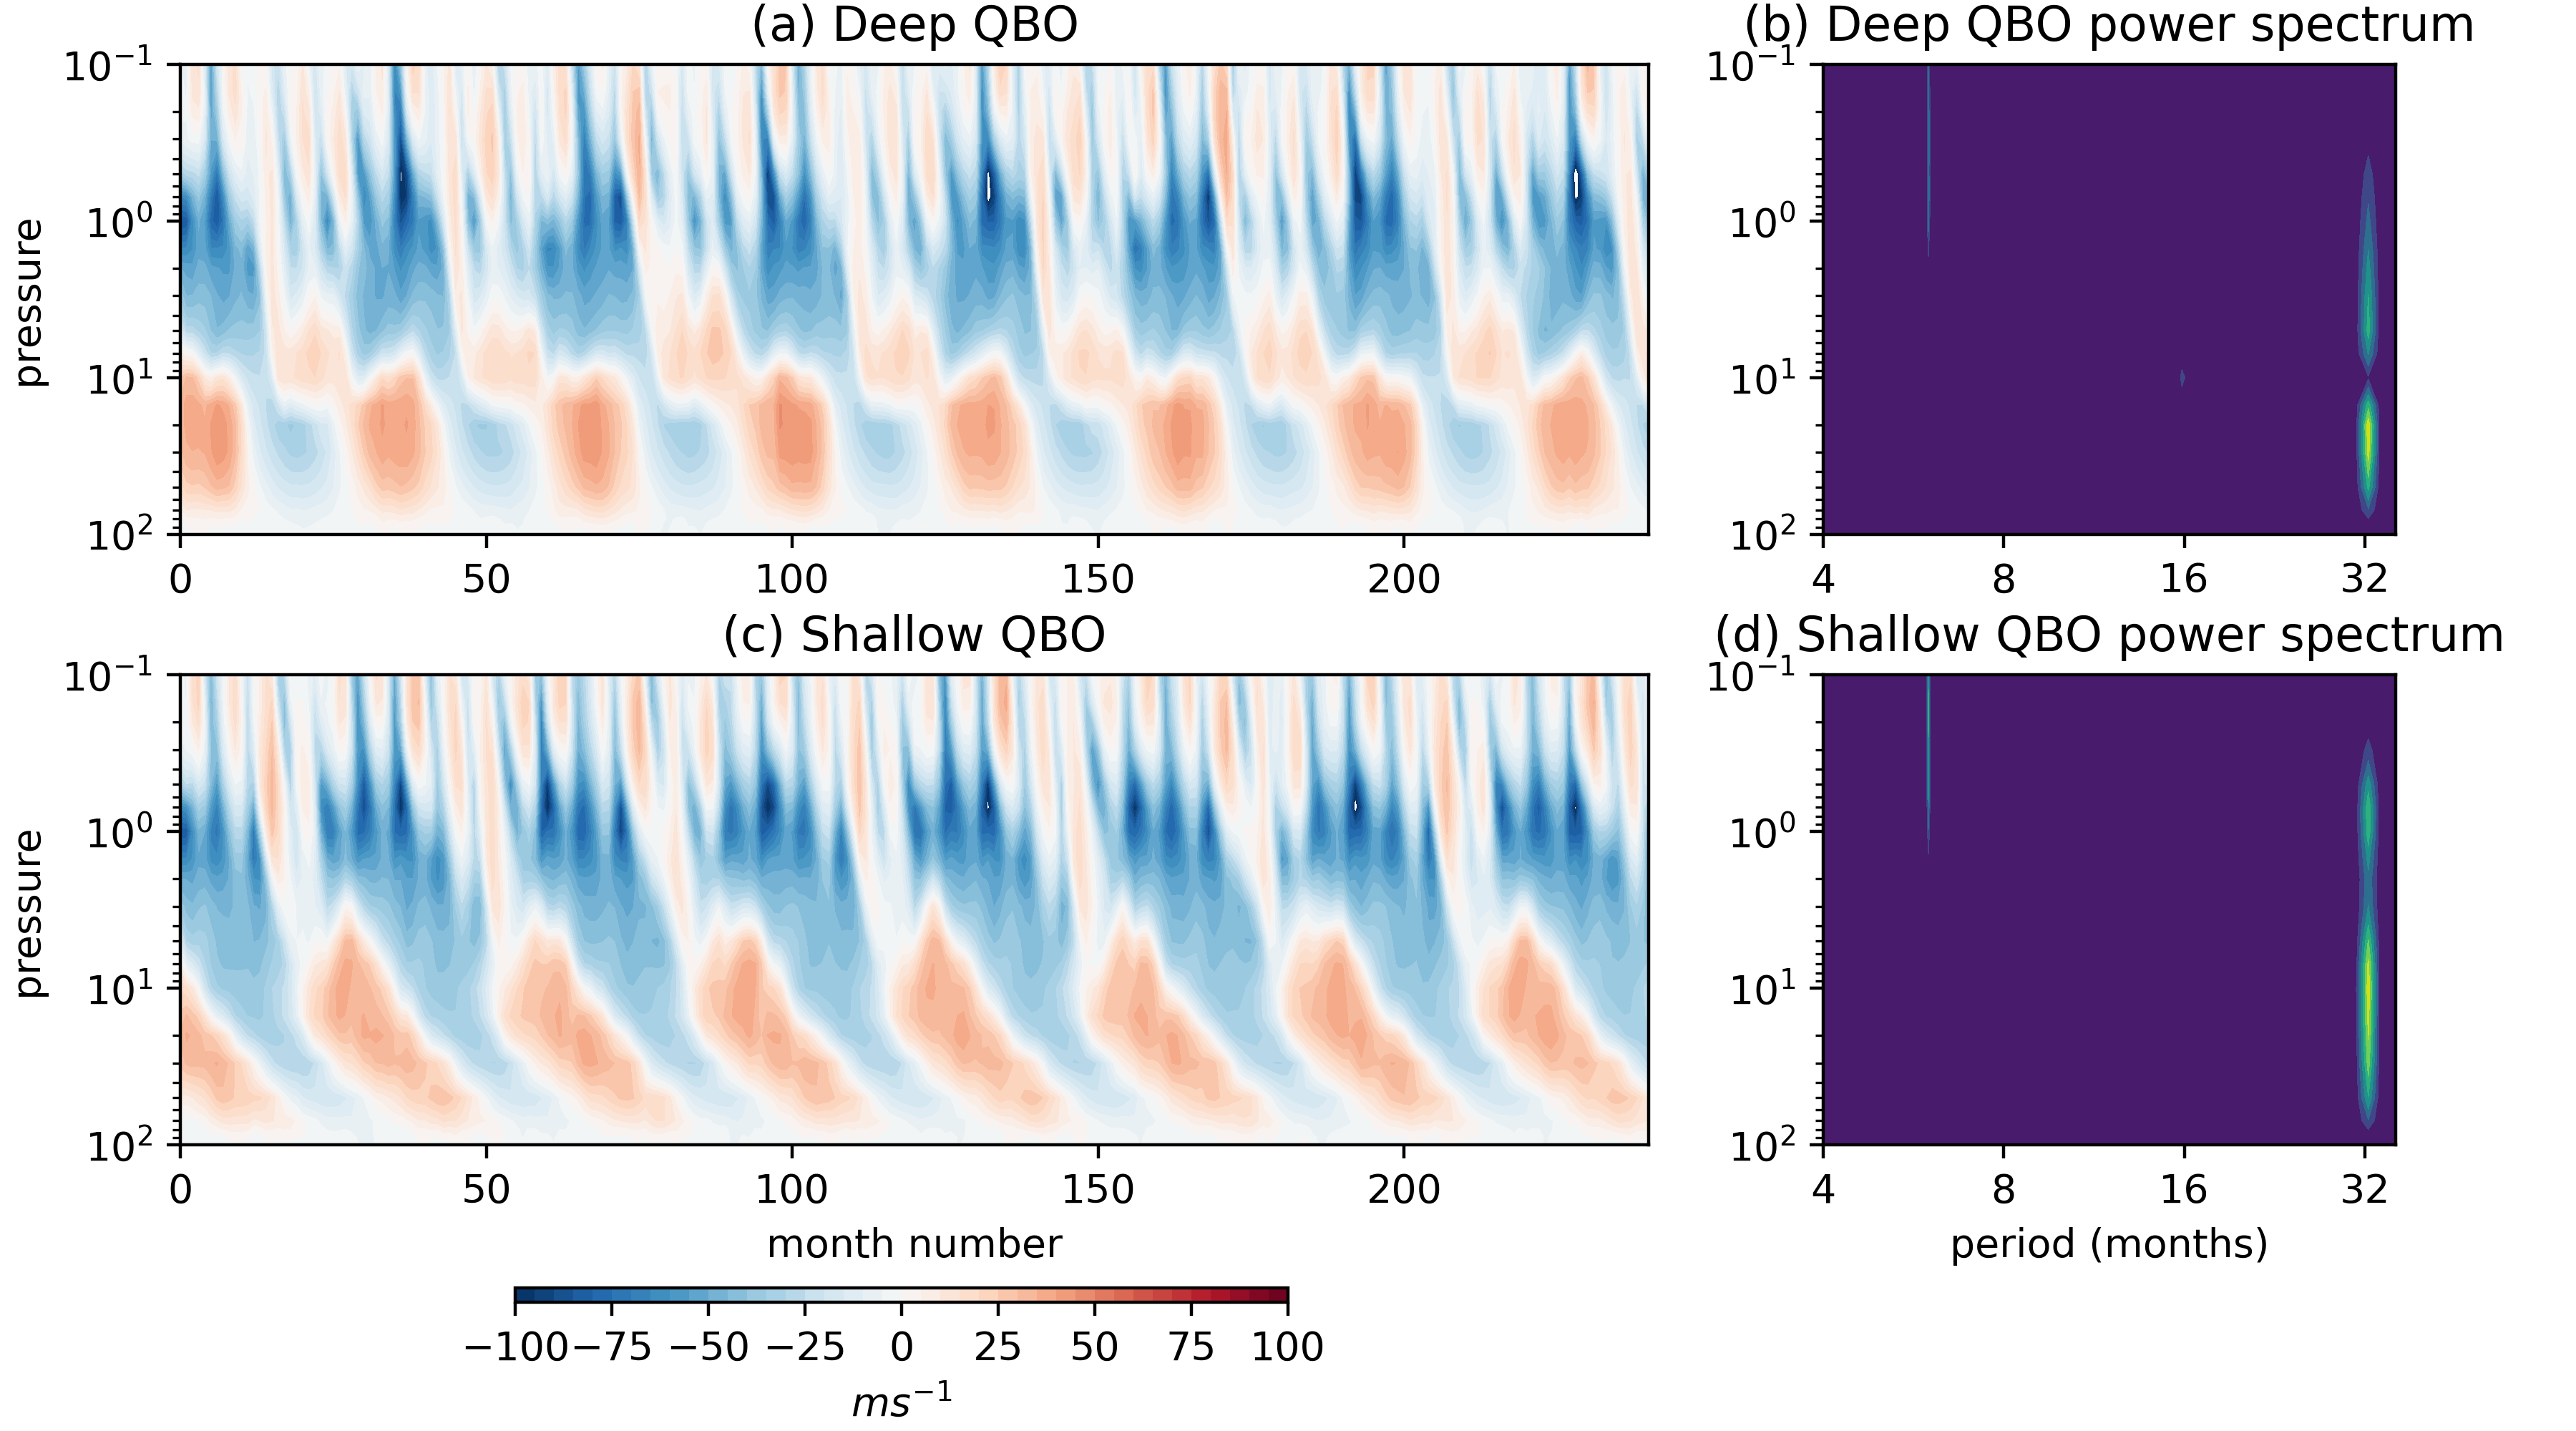
\includegraphics[width = \linewidth]{Figures/Figures-deepQBO/experiment_QBOs.png}
\caption[Equatorial ZMZW time-height profiles from QBO nudging experiments]{20 year sample of ZMZW averaged between 5$^{\circ}$\,S--5$^{\circ}$\,N latitude from the deep (\textbf{a}) and shallow (\textbf{c}) QBO experiments. Horizontal dashed lines on (a) and (c) denote the xxhPa and 90hPa pressure levels between which we implement nudging towards the idealised wind in each experiment.}
\label{fig:experiment_QBOs}
\end{center}
\end{figure}

While the simulations' QBO reflects some of the main characteristics of the target nudging winds, there is a notable asymmetry in the amplitudes of the two QBO phases in both experiments with the westerly phase amplitude appearing larger in all QBO cycles throughout each simulation. This is an unexpected result - We defined the target nudging field using equation \ref{eq:imposed_U} which ensures each phase of the idealised QBO exhibits identical magnitude (i.e. $F(z)$ in equation \ref{eq:imposed_U} is constant in time). To examine this asymmetry further, we analyse the timeseries of simulated and idealised winds on individual pressure levels to identify potential biases (Figures \ref{fig:winds_on_levs_deep} and \ref{fig:winds_on_levs_shallow}). In the deep experiment (figure \ref{fig:winds_on_levs_deep}) the easterly phase of the QBO is in good agreement with the idealised winds on each of the pressure levels sampled. In contrast, the magnitude of the westerly phase resulting from the simulation is systematically over-represented compared to the nudging winds. This effect is apparent throughout much of the mid-stratosphere (10hPa-50hPa) and suggests the possibility of a westerly momentum forcing term in the model which acts to override the influence of the nudging scheme. This in turn may suggest that our selection of nudging timescale, $\tau$ = 6 hours, is too long in relation to other forcing terms which act on shorter timescales. The effect is less pronounced in the shallow experiment with only the QBO at 50hPa exhibiting notable over-representation in westerly amplitude. The source of additional forcing term is unclear but is likely closely associated with kelvin wave forcing as this is the primary source of the westerly QBO phase (see section \ref{sec:equatorial_strat}). While this bias does lead to marginal asymmetries in QBO phases, the desired vertical structures is obtained in both experiments which is the focus of this study and therefore we proceed with the simulations for analysis of QBO teleconnections in the next section. The possible detrimental effect of this amplitude bias is that NH winters in which we study teleconnections may preferentially occur under one QBO phase more than the other. As a result, in all future analysis of these simulations we note the number of NH winters exhibiting each QBO phase and only draw major conclusions in cases where their abundance is comparable. The result from figures \ref{fig:winds_on_levs_deep} and \ref{fig:winds_on_levs_shallow} may also indicate the suitability of a shorter nudging timescale for future nudged QBO experiments using this model setup than that recommended by the MetOffice Unified Model documentation (xxxx) but further simulations are required to confirm this.

\begin{figure}[h!]
\begin{center}
\noindent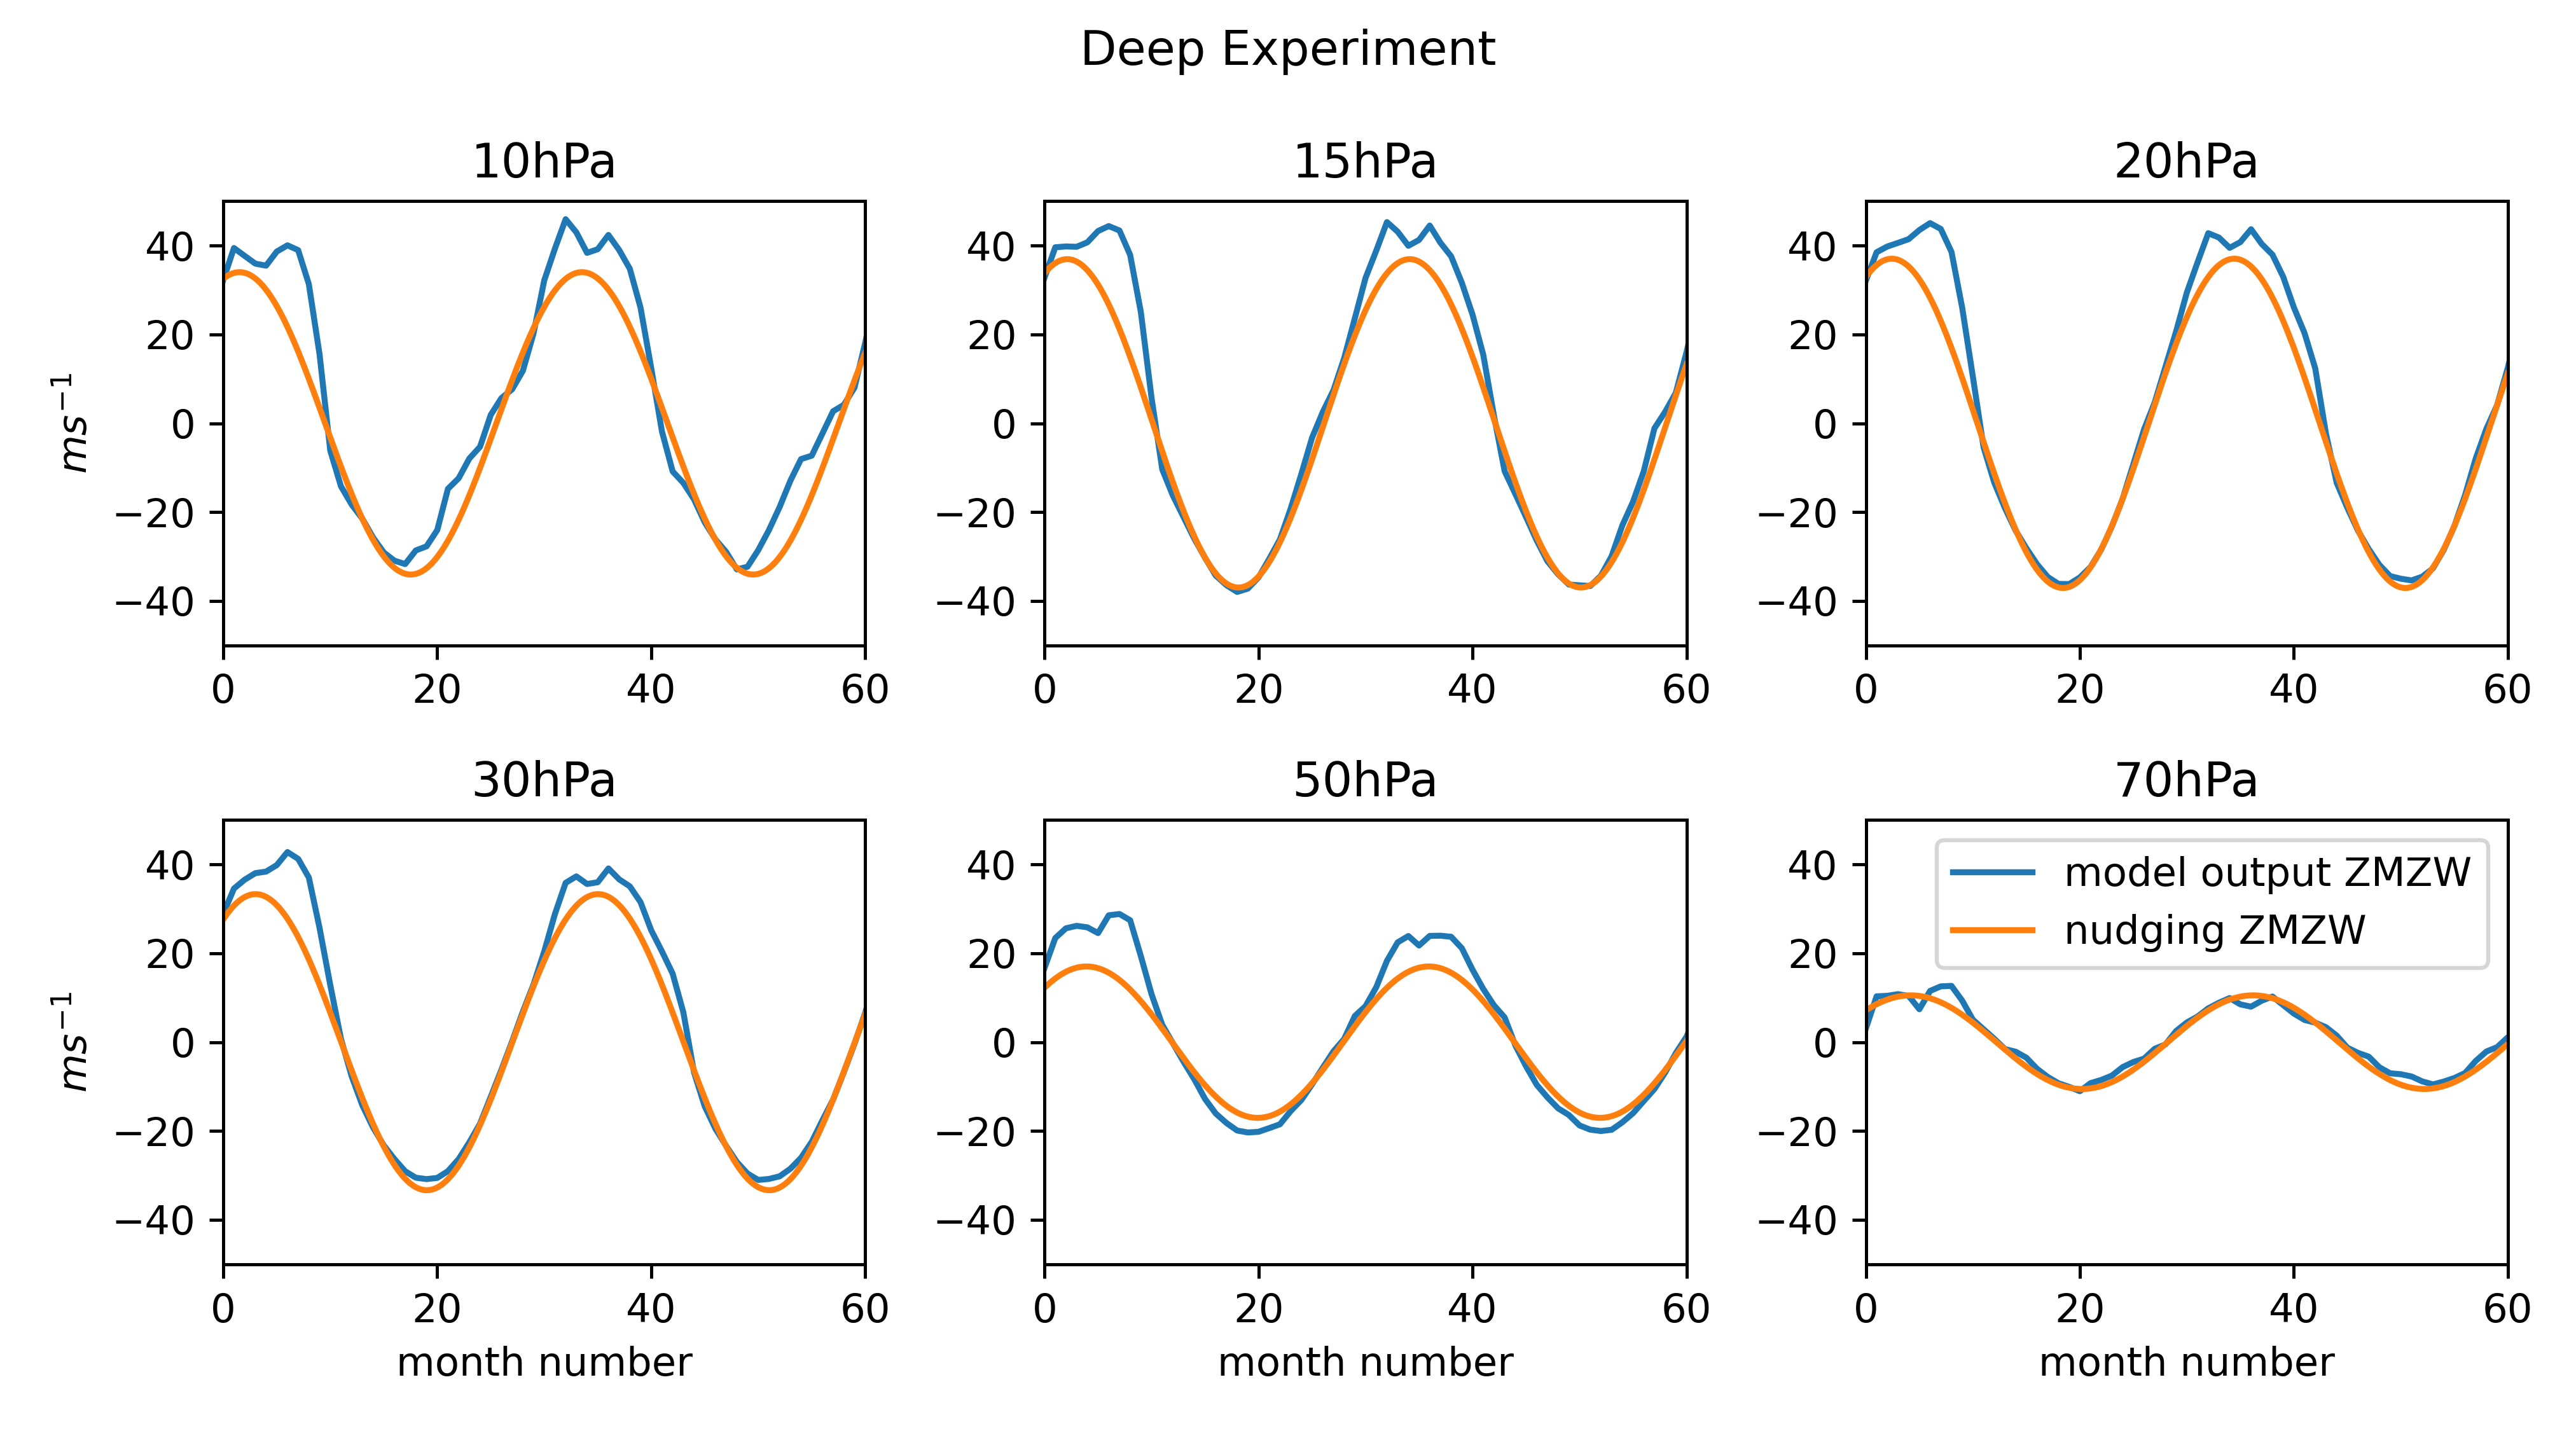
\includegraphics[width = 0.95\linewidth]{Figures/Figures-deepQBO/winds_on_lev_nudging_deep.png}
\caption[Equatorial ZMZW time-height profiles from QBO nudging experiments]{5 year sample of ZMZW on individual pressure levels averaged between 5$^{\circ}$\,S--5$^{\circ}$\,N latitude from the deep QBO experiments (blue) and the Idealised wind field used for nudging in the same experiment (orange).}
\label{fig:winds_on_levs_deep}
\end{center}
\end{figure}

\begin{figure}[h!]
\begin{center}
\noindent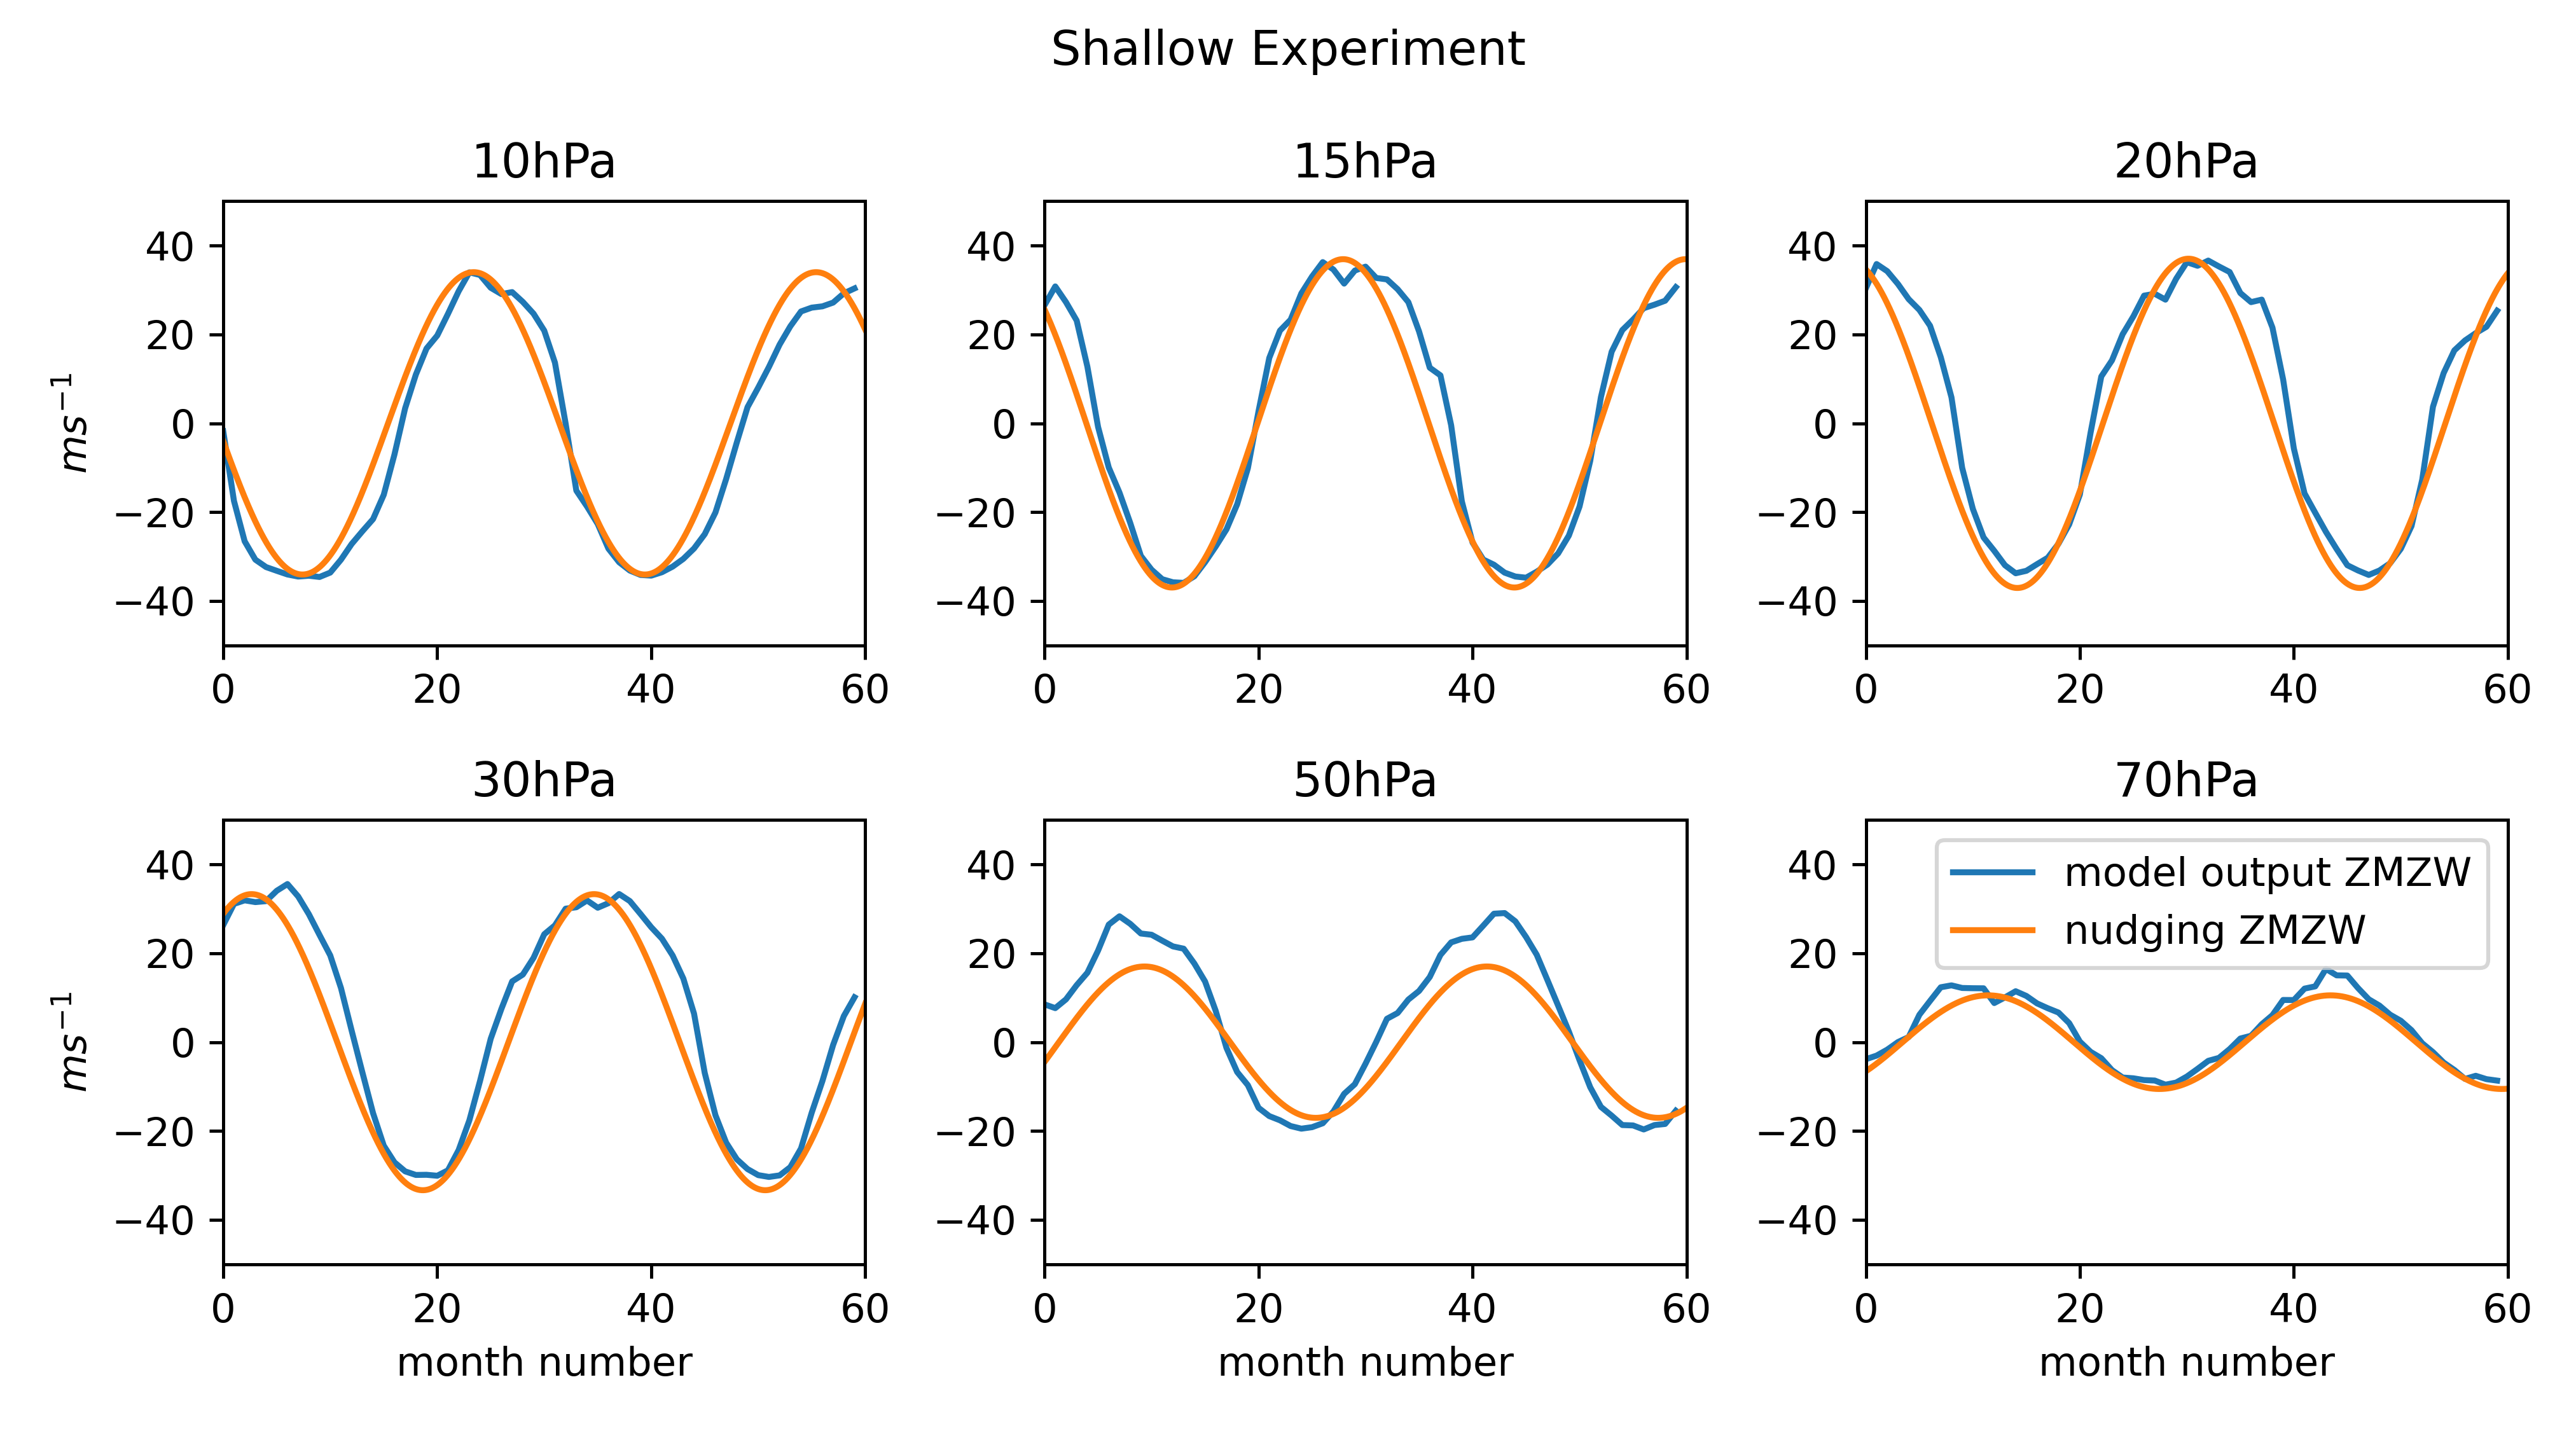
\includegraphics[width = 0.95\linewidth]{Figures/Figures-deepQBO/winds_on_lev_nudging_shallow.png}
\caption[Equatorial ZMZW time-height profiles from QBO nudging experiments]{Like figure \ref{fig:winds_on_levs_deep} for the shallow QBO experiment.}
\label{fig:winds_on_levs_shallow}
\end{center}
\end{figure}


\section{Upper Atmosphere Characteristics}

In addition to the imposed QBO states, both experiments also exhibit variations in ZMZW on the 1hPa level and above corresponding to a period of $\sim$ 6 months which indicates the presence of an SAO like variation (see figure \ref{fig:experiment_QBOs}). Previous work suggests a key role for this region in equator-vortex teleconnections (e.g. brown et al. xxxx) as well as elements of synchronisation between the QBO and SAO \citep{kuaiNonstationary2009}. As each experiment imposes significantly different QBO states, features of SAO in both experiments may play a key role in dictating responses from the vortex, troposphere and surface. There are notable differences in the SAO winds across the two experiments apparent from the wind fields above 10hPa in figures \ref{fig:experiment_QBOs}a and d: The deep experiment exhibits stronger easterly SAO phases than in the shallow experiment and the westerly phase is significantly more prominent in the shallow experiment. These differences can be formally diagnosed through analysis of climatological wind profiles from each experiment. latitude-height ZMZW climatologies for NH winter (Dec-Mar) during predominantly the easterly phase of the SAO (figure \ref{fig:climatologies_experiments}) confirms significant differences in mean winds above 1hPa indicating that the shallow experiment's easeterly amplitude is greater than that of the deep experiment. 

\begin{figure}[h!]
\begin{center}
\noindent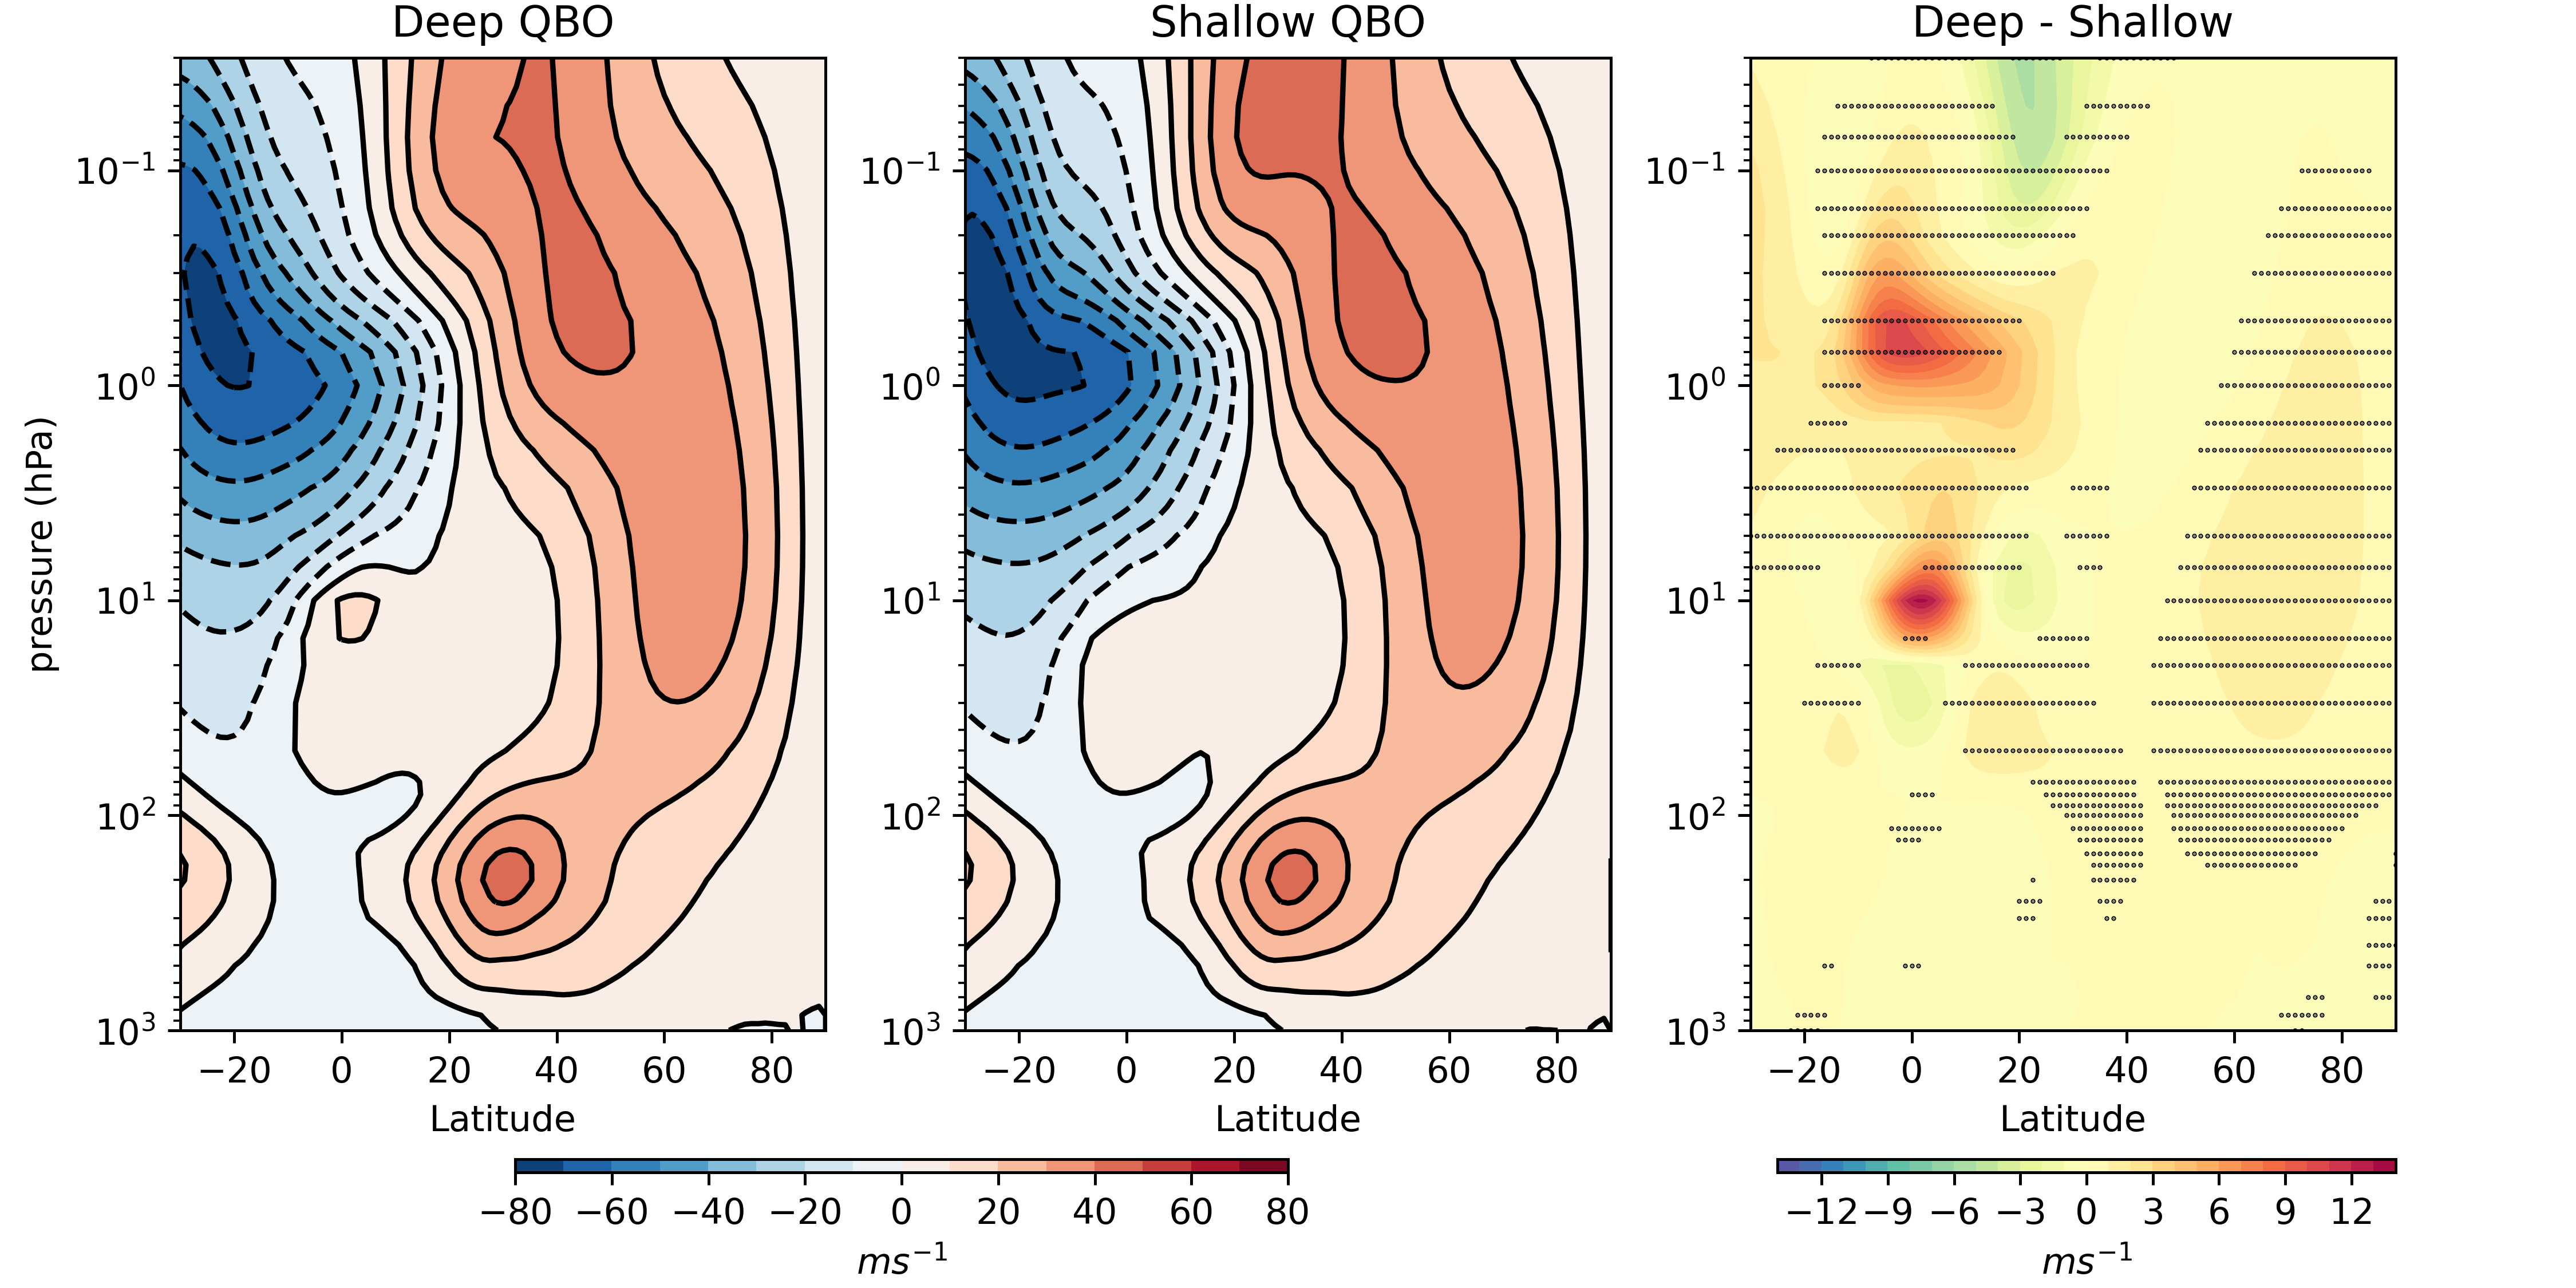
\includegraphics[width = \linewidth]{Figures/Figures-deepQBO/DJF_climatologies.png}
\caption[Equatorial ZMZW time-height profiles from QBO nudging experiments]{20 year sample of ZMZW averaged between 5$^{\circ}$\,S--5$^{\circ}$\,N latitude from the deep (\textbf{a}) and shallow (\textbf{c}) QBO experiments. Horizontal dashed lines on (a) and (c) denote the xxhPa and 90hPa pressure levels between which we implement nudging towards the idealised wind in each experiment.}
\label{fig:climatologies_experiments}
\end{center}
\end{figure}

Additional analysis of the climatological seasonal cycle in equatorial winds (figure \ref{fig:experiment_SAOs}) reveals further differences in simulation SAOs: the westerly phase of the SAO appearing in early NH winter (Sep-Nov), which is attributed to the dissipation of Kelvin waves smaller scale inertia-gravity waves \citep{Dunkerton1982, Hitchman1988}, is significantly weaker and exhibits less vertical extent in the deep experiment compared to the shallow. The timing of phase transitions from westerly to easterly in early NH winter (denoted by the climatological zero wind line on approximately the 0.1hPa level) is also marginally later in the shallow experiment. These differences in the extent of the westerly SAO phase could play a key role in equator-vortex interactions in each experiment as these features, particularly phase transition timings, have been shown to associate with the occurrence of SSWs \citep{JGray2001, Hamilton}. The results from figures \ref{fig:climatologies_experiments} and \ref{fig:experiment_SAOs} highlight the potential impact that the degree of vertical coherence in the QBO may have have on the characteristics of the upper atmosphere. The role these SAO variations play in teleconnections with the vortex, the troposphere and surface is explored further in section xxxx.

\begin{figure}[h!]
\begin{center}
\noindent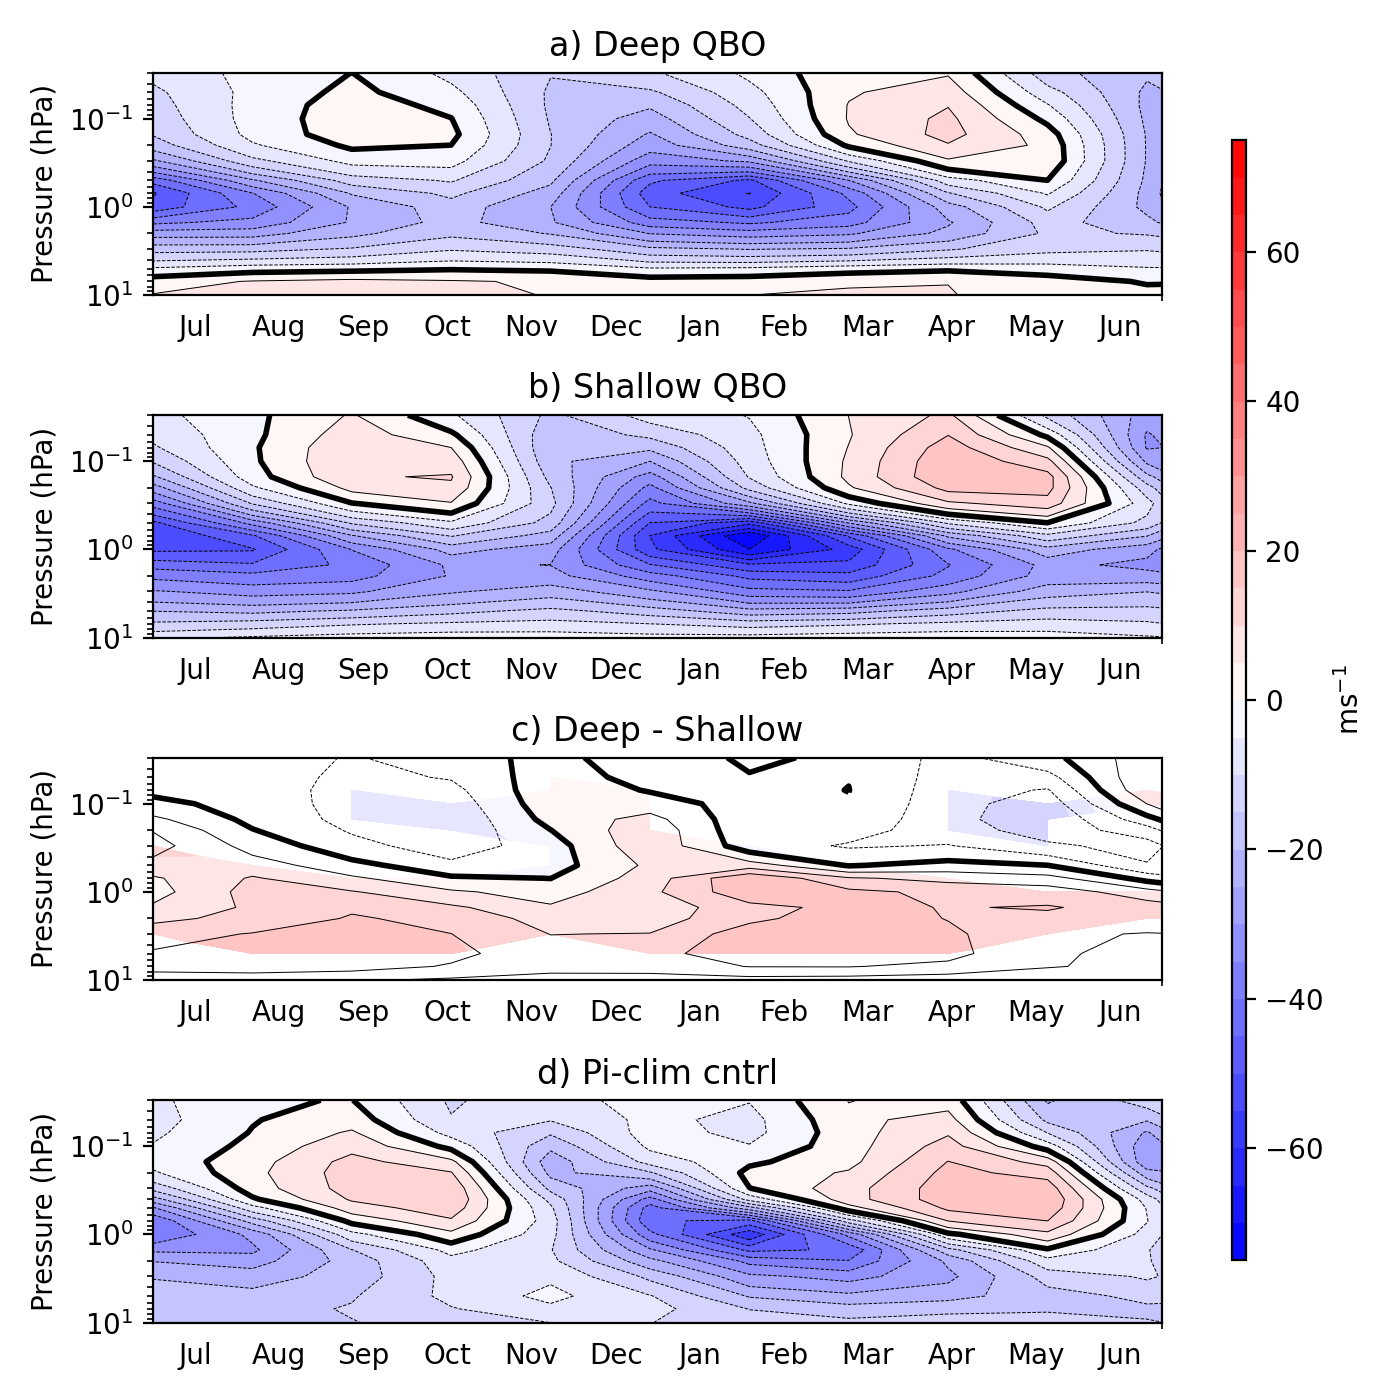
\includegraphics[width = 0.7\linewidth]{Figures/Figures-deepQBO/SAO_seasonal_cycles.png}
\caption[Climatological seasonal cycle of equatorial ZMZW in QBO experiments]{Climatological seasonal cycle of ZMZW averaged between 5$^{\circ}$\,S--5$^{\circ}$\,N latitude from the deep (\textbf{a}) and shallow (\textbf{b}) QBO experiments. Panel \textbf{c} shows climatological differences between deep and shallow seasonal cycles. Black dots on (c) denote differences significant to the 95\% level under a 2-tailed student's t-test.}
\label{fig:experiment_SAOs}
\end{center}
\end{figure}


\section{QBO teleconnections}
So far, we have shown that both experiments exhibit the desired vertical structure in the QBO as well as the potential influence of such structures on SAO variability. The focus of this study however, is the different teleconnections that arise between the equator and other parts of the climate system such as that with the NAO demonstrated in \cite{andrewsObserved2019}. Next, we analyse composites of common diagnostics of climate variability under different QBO conditions in each experiment to compare the nature of teleconnections. 

Figure \ref{fig:HT_deep} shows a measure of the strength of the Holton-Tan effect in the deep experiment -  composites of NH winter (Dec-Mar) ZMZW anomalies under QBO-east (QBOE) and QBO-west (QBOW) defined on various pressure levels. At each pressure level, the anomaly composites for each phase (figure \ref{fig:HT_deep}, left and middle columns) exhibit vertically coherent anomalies between 10hPa and 100hPa. This is consistent with figure \ref{fig:experiment_QBOs} which shows agreement between all mid-stratosphere levels in QBO phase. In the SAO region (above 10hPa), composites for both QBOE and QBOW phases exhibit large anomalies of the opposite sign of the QBO phase below. This is consistent with the idea of vertically coherent QBO phases filtering out waves with the same phase speed direction as the QBO and permitting wave forcing of the opposite phase speed into the lower mesosphere leading to anomalies of the opposite sign. There is also a negative response in the polar vortex to the westerly QBO at all sampled levels (figure \ref{fig:HT_deep}, middle row). This is another unexpected result - the traditional HT effect explored in chapter 3 would predict the westerly phase of the QBO to be associated with a strengthened vortex as vertically propagating planetary waves were permitted over greater latitudinal range according to the Charney-Drazin criterion. Instead, this result may indicate an important role for the SAO in the response of the vortex of the QBO. Indeed, the composite difference (QBOE-QBOW) shows a significantly strengthened vortex ($\sim 8 ms^{-1}$ composite difference) as well as anomalously westerly SAO winds which is consistent with mechanisms proposed in \cite{gray}

Additionally, the composite differences show a significant tropospheric response in the subtropical jet region (xx-xx) with the same sign as the QBO anomaly. This may be evidence for the so called 'subtropical path' hypothesised in \cite{graySurface2018} by which the QBO influences tropospheric and surface variability directly (as opposed to via modulation of the vortex). This pathway is analysed in closer detail in the foll


\begin{figure}[h!]
\begin{center}
\noindent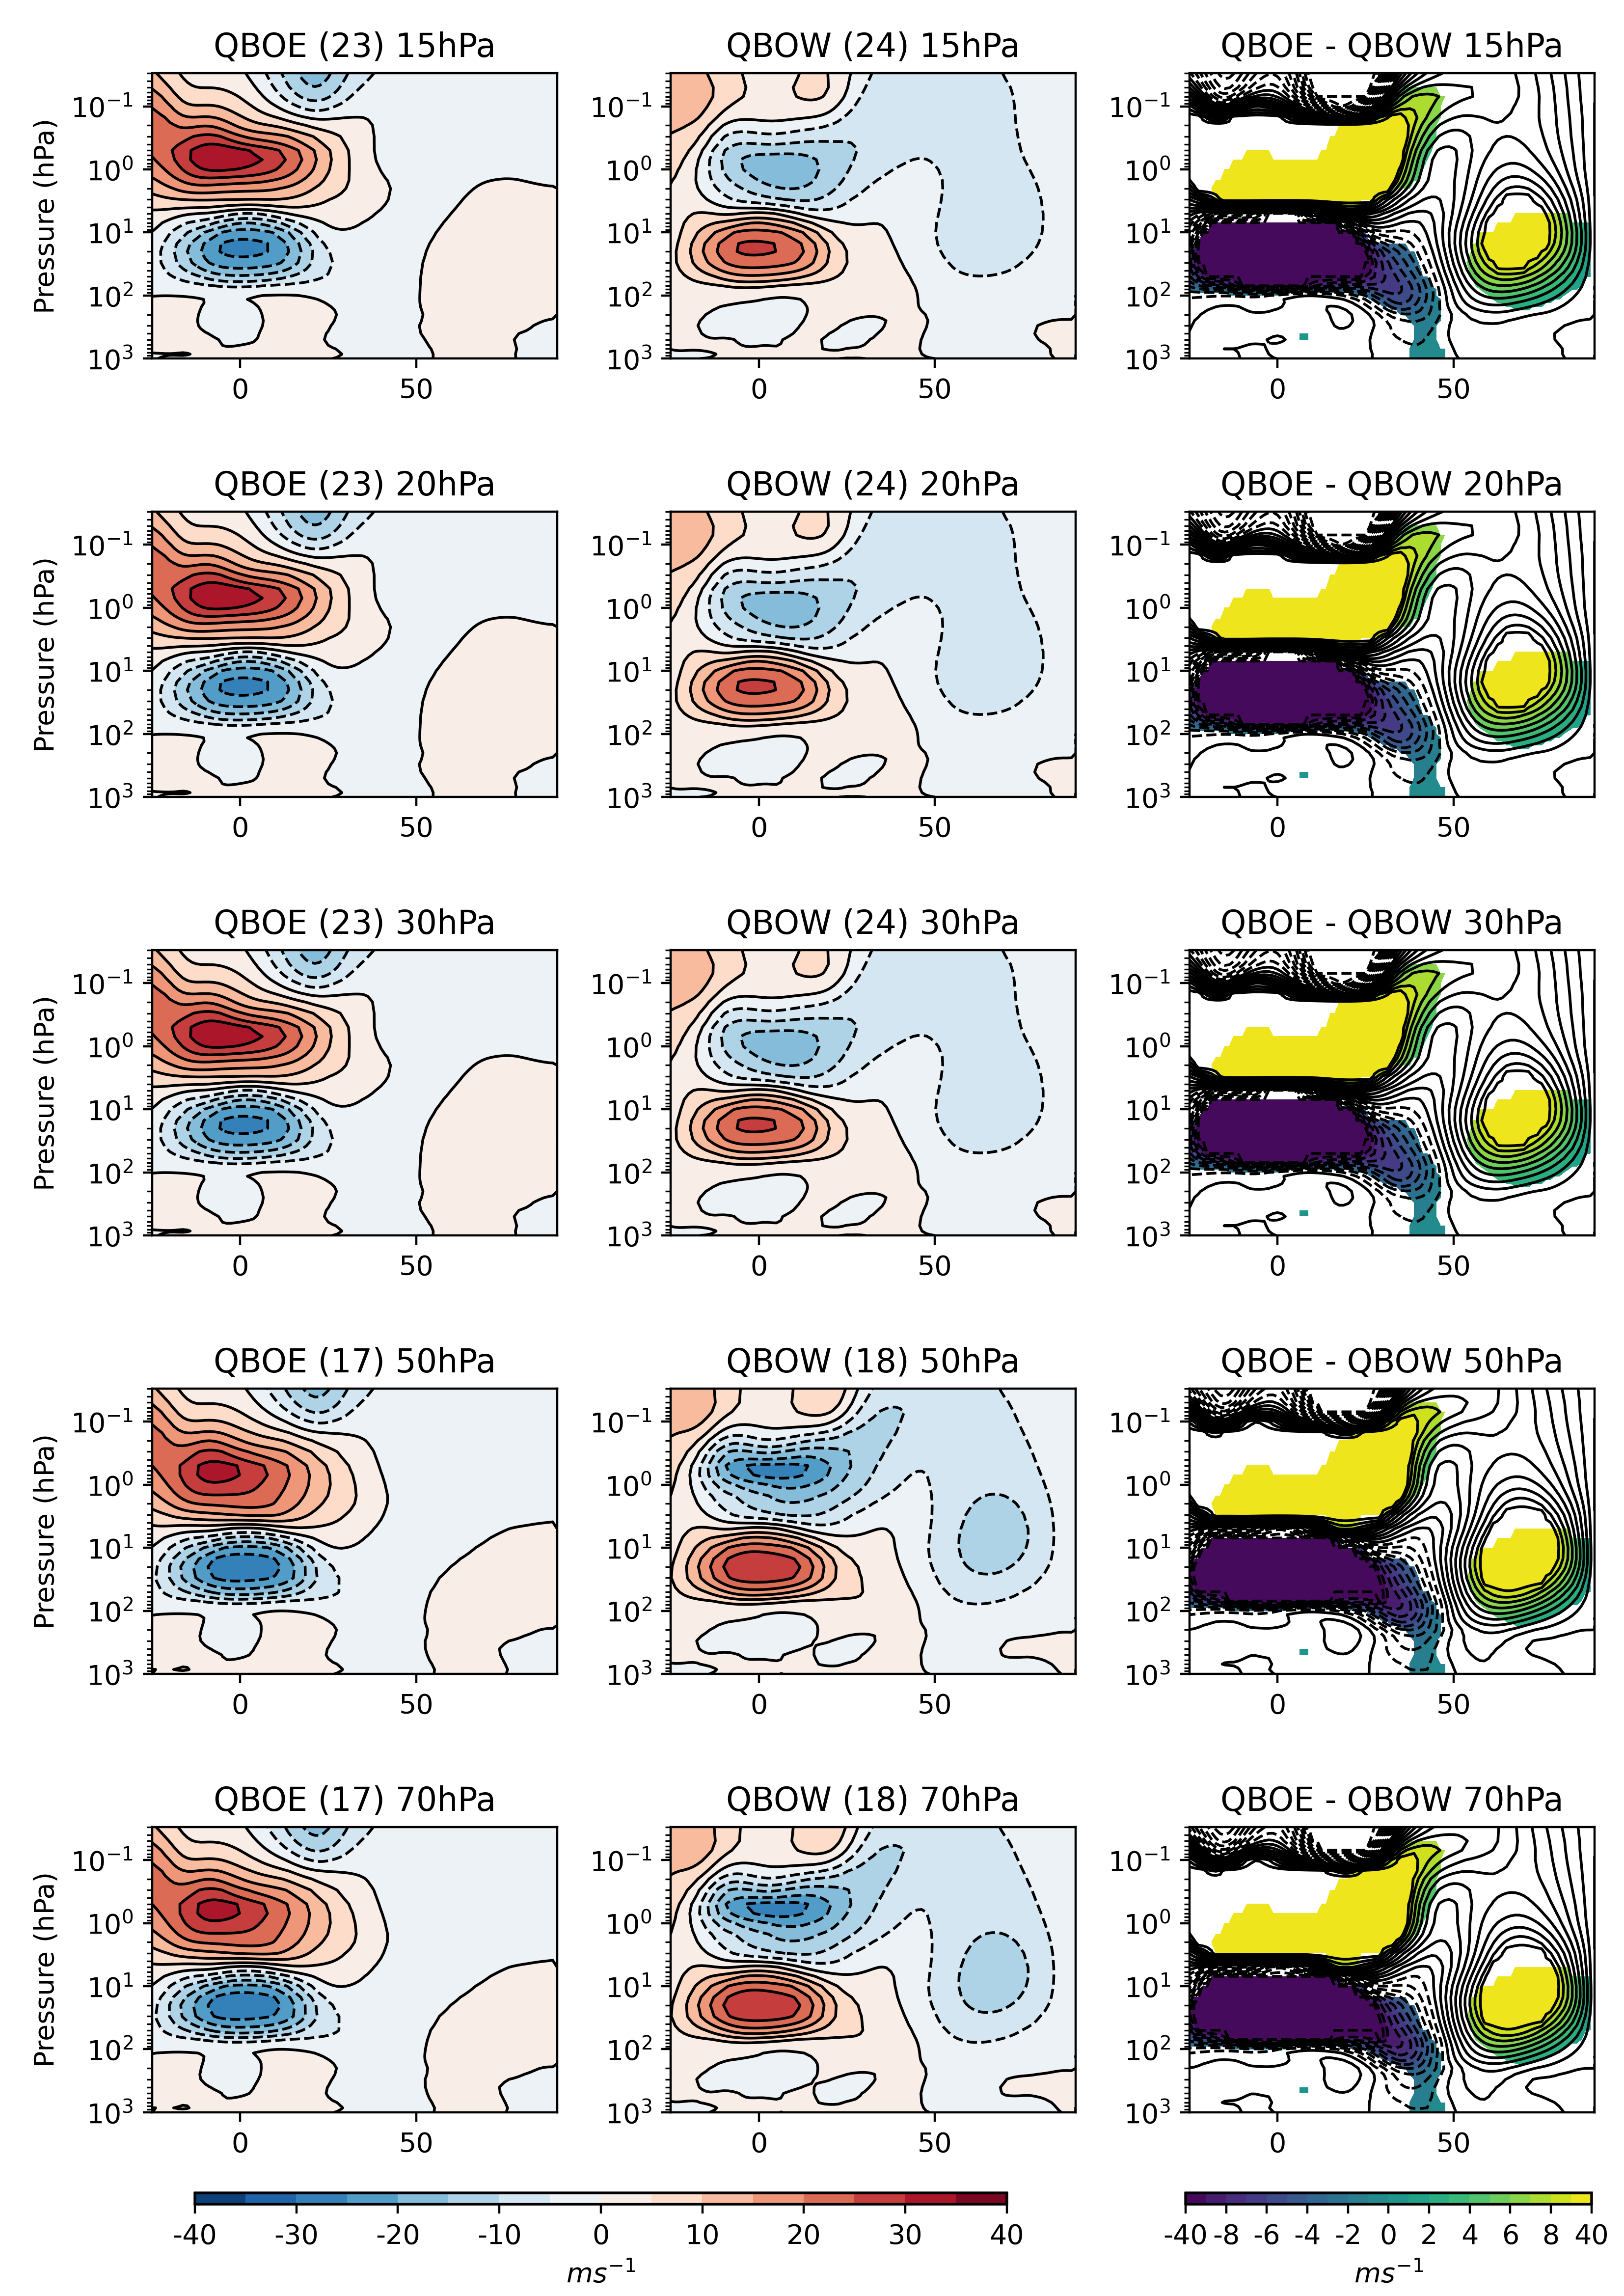
\includegraphics[width = \linewidth]{Figures/Figures-deepQBO/ZMZW_composites_QBO_phases_U_d_higher_DJFMQBO_vs_DJFM_70hPa_5thresh.png}
\caption[]{Dec-Mar ZMZW anomaly composites for QBO East (left column), QBO West (middle column) phases and composite differences (QBOE - QBOW, right column). The QBO phase is defined as any Dec-Mar equatorial ($5^{\circ}$\ S--$5^{\circ}\ $N average) ZMZW that exceeds a magnitude of 5\ m\,s$^{-1}$ on individual levels (which are indicated in sub-figure titles). Numbers in parentheses indicate the number of winters of each phase that make up the composite. Coloured shading in the right column indicates ZMZW differences significant above the 95\% confidence level under a 2 tail student’s t-test.}
\label{fig:HT_deep}
\end{center}
\end{figure}

ZMZW anomaly composites for the shallow experiment (figure 

\begin{figure}[h!]
\begin{center}
\noindent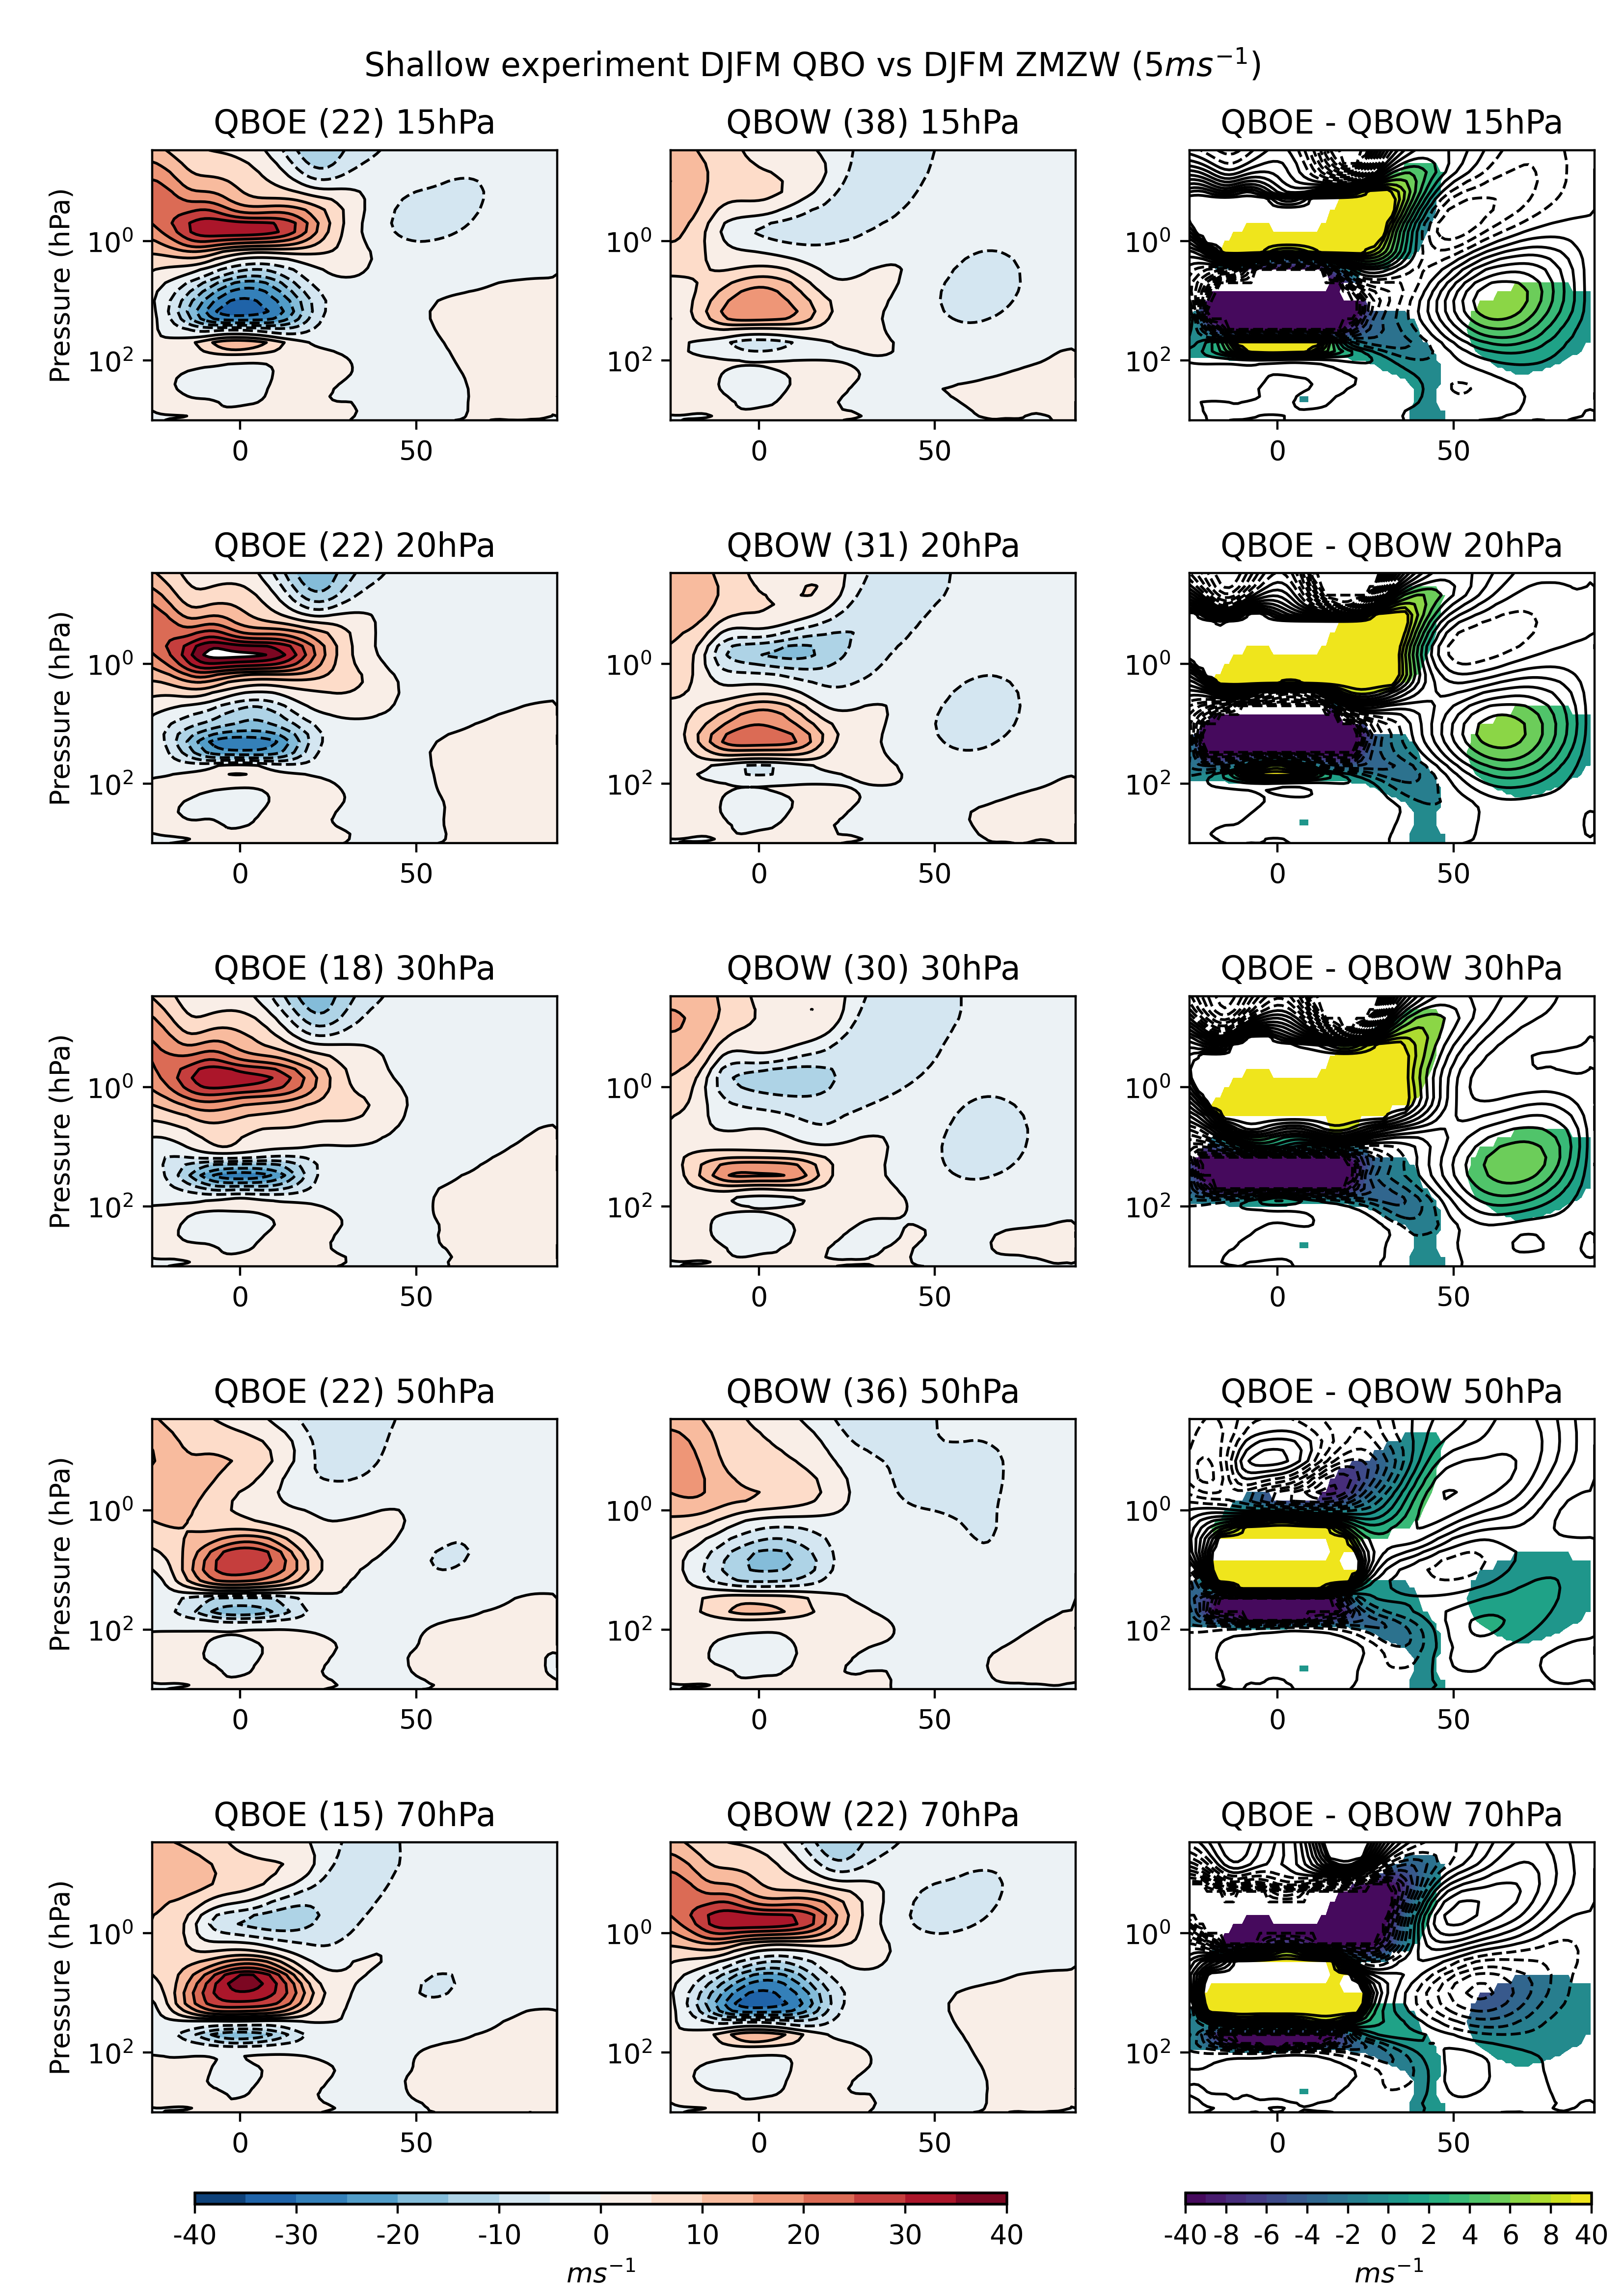
\includegraphics[width = \linewidth]{Figures/Figures-deepQBO/ZMZW_composites_QBO_phases_U_s_DJFMQBO_vs_DJFM_70hPa_5thresh.png}
\caption[Climatological seasonal cycle of equatorial ZMZW in QBO experiments]{Like figure \ref{fig:HT_deep} for the shallow experiment}
\label{fig:HT_deep}
\end{center}
\end{figure}





\begin{figure}[h!]
\begin{center}
\noindent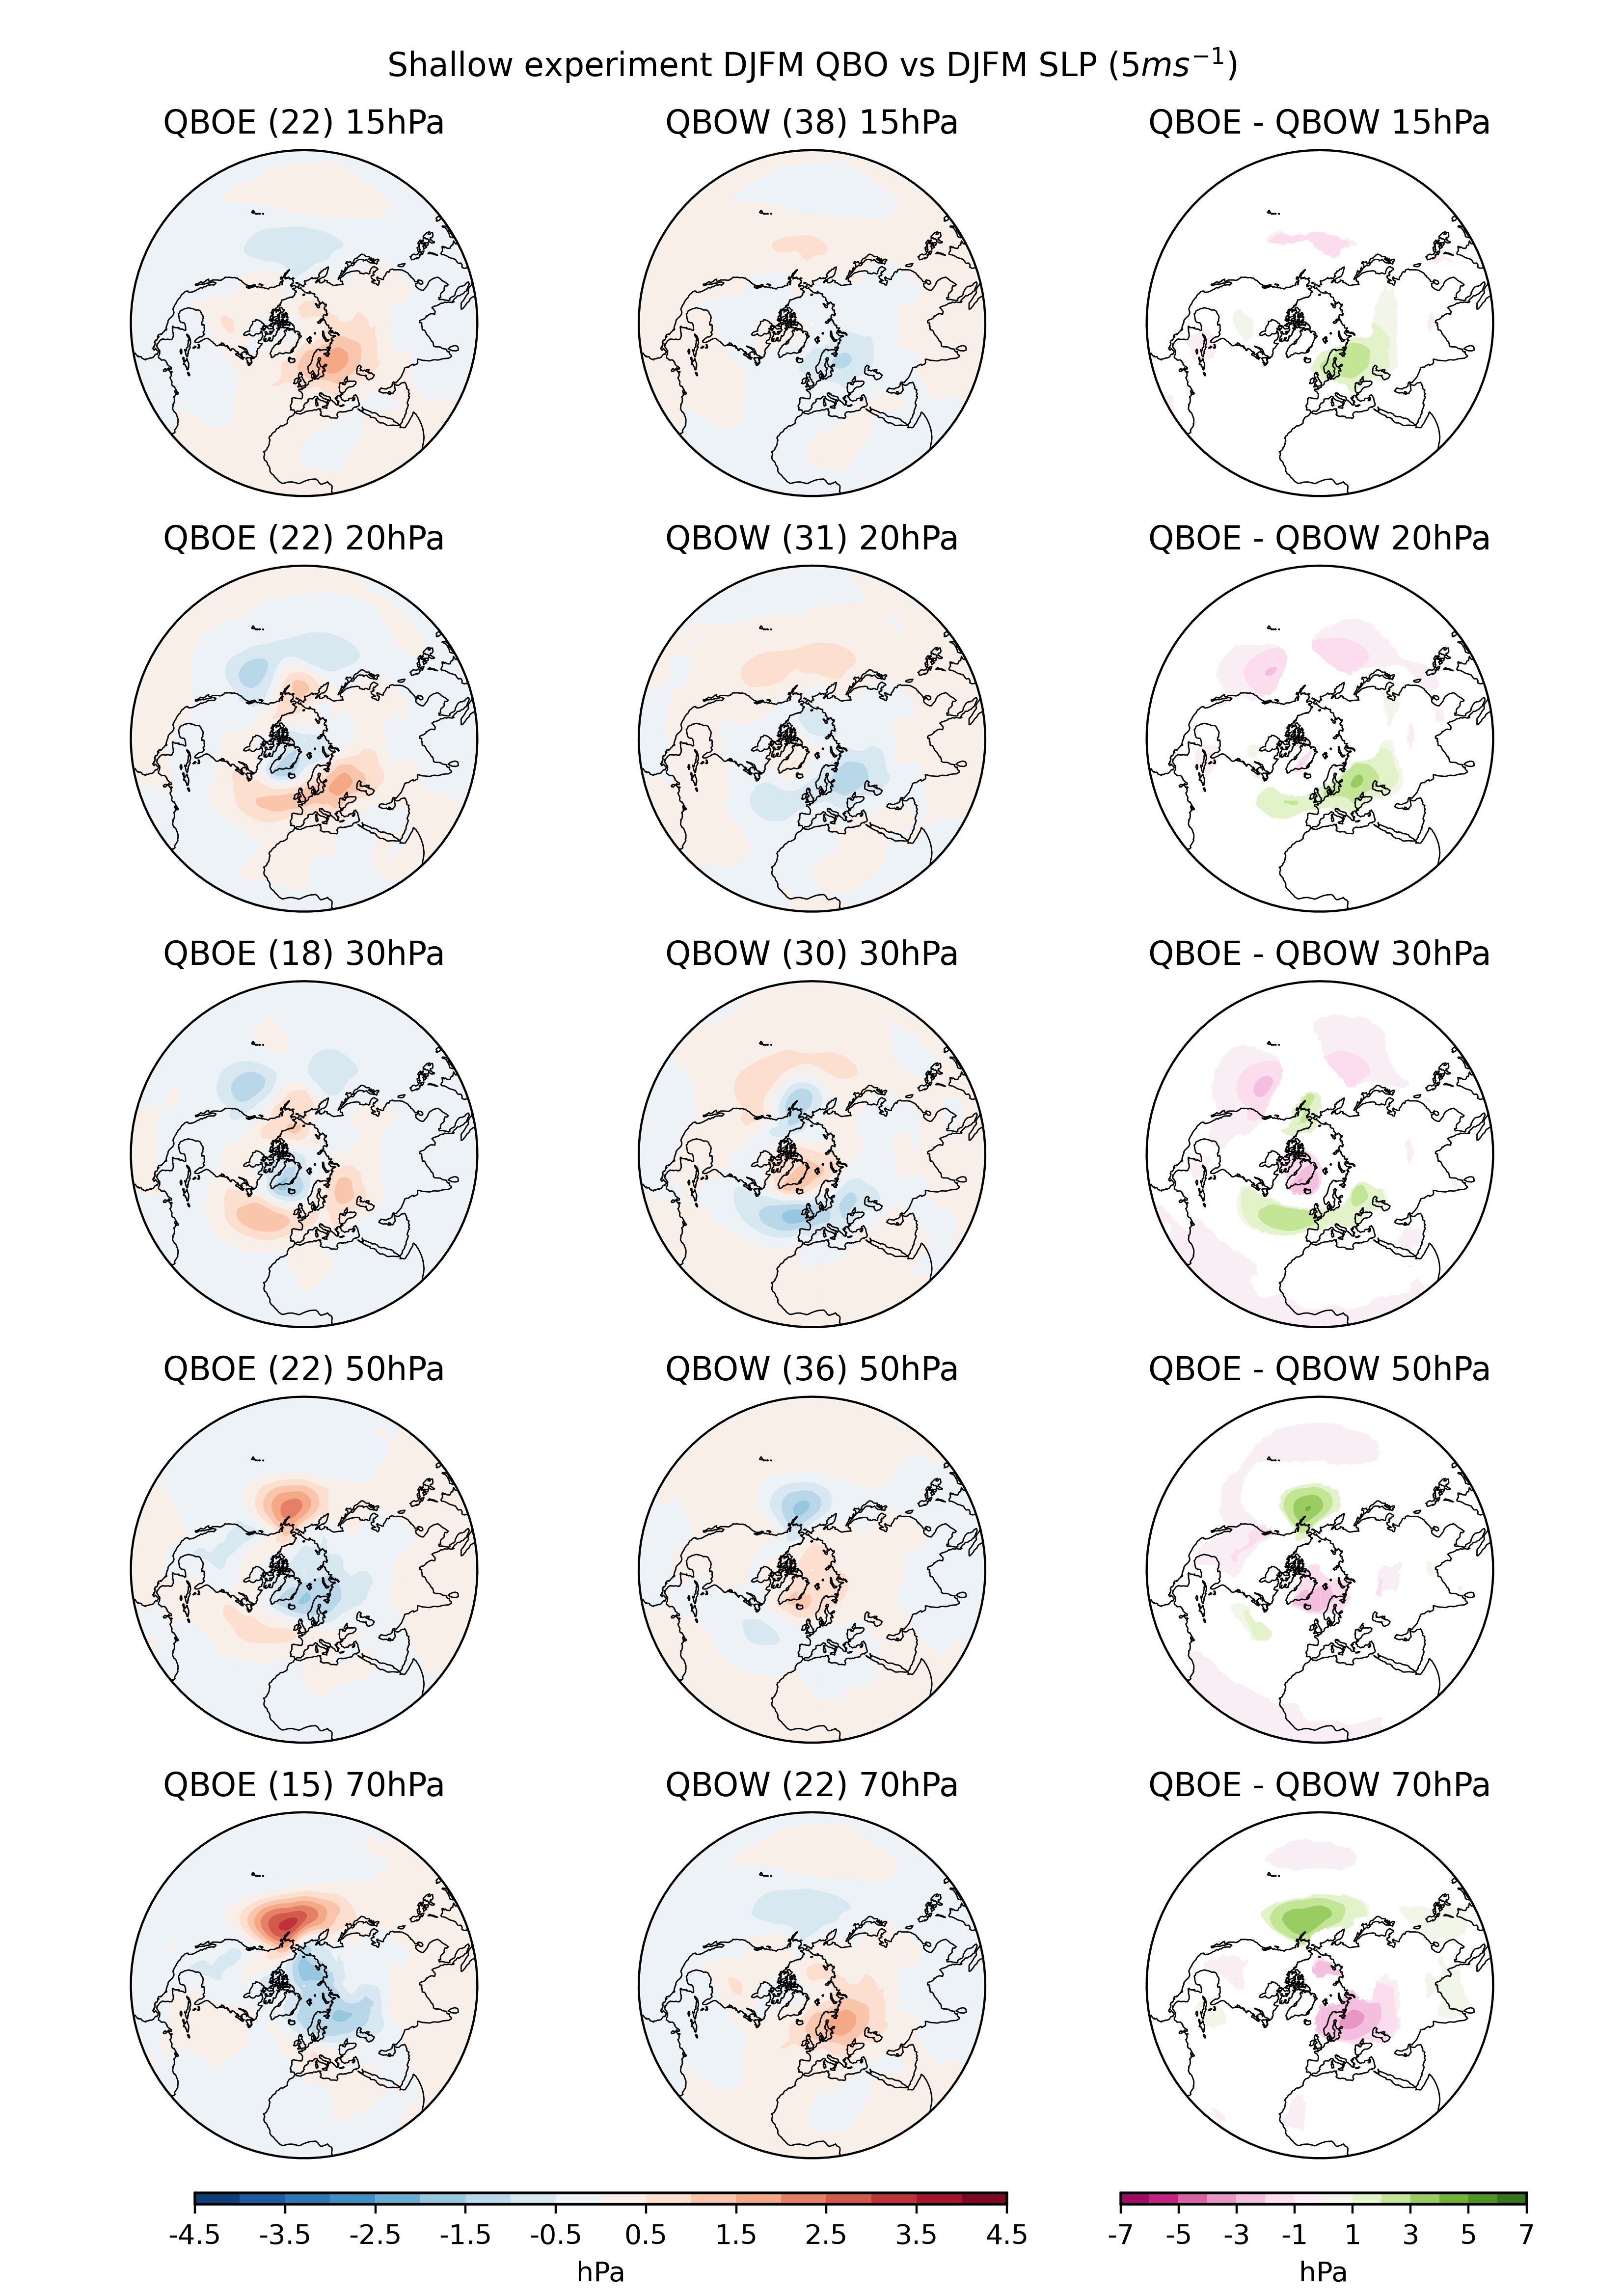
\includegraphics[width = \linewidth]{Figures/Figures-deepQBO/SLP_composites_QBO_phases_s_DJFMQBO_vs_DJFM_70hPa_5thresh.png}
\caption[Climatological seasonal cycle of equatorial ZMZW in QBO experiments]{Climatological seasonal cycle of ZMZW averaged between 5$^{\circ}$\,S--5$^{\circ}$\,N latitude from the deep (\textbf{a}) and shallow (\textbf{b}) QBO experiments. Panel \textbf{c} shows climatological differences between deep and shallow seasonal cycles. Black dots on (c) denote differences significant to the 95\% level under a 2-tailed student's t-test.}
\label{fig:experiment_SAOs}
\end{center}
\end{figure}


\begin{figure}[h!]
\begin{center}
\noindent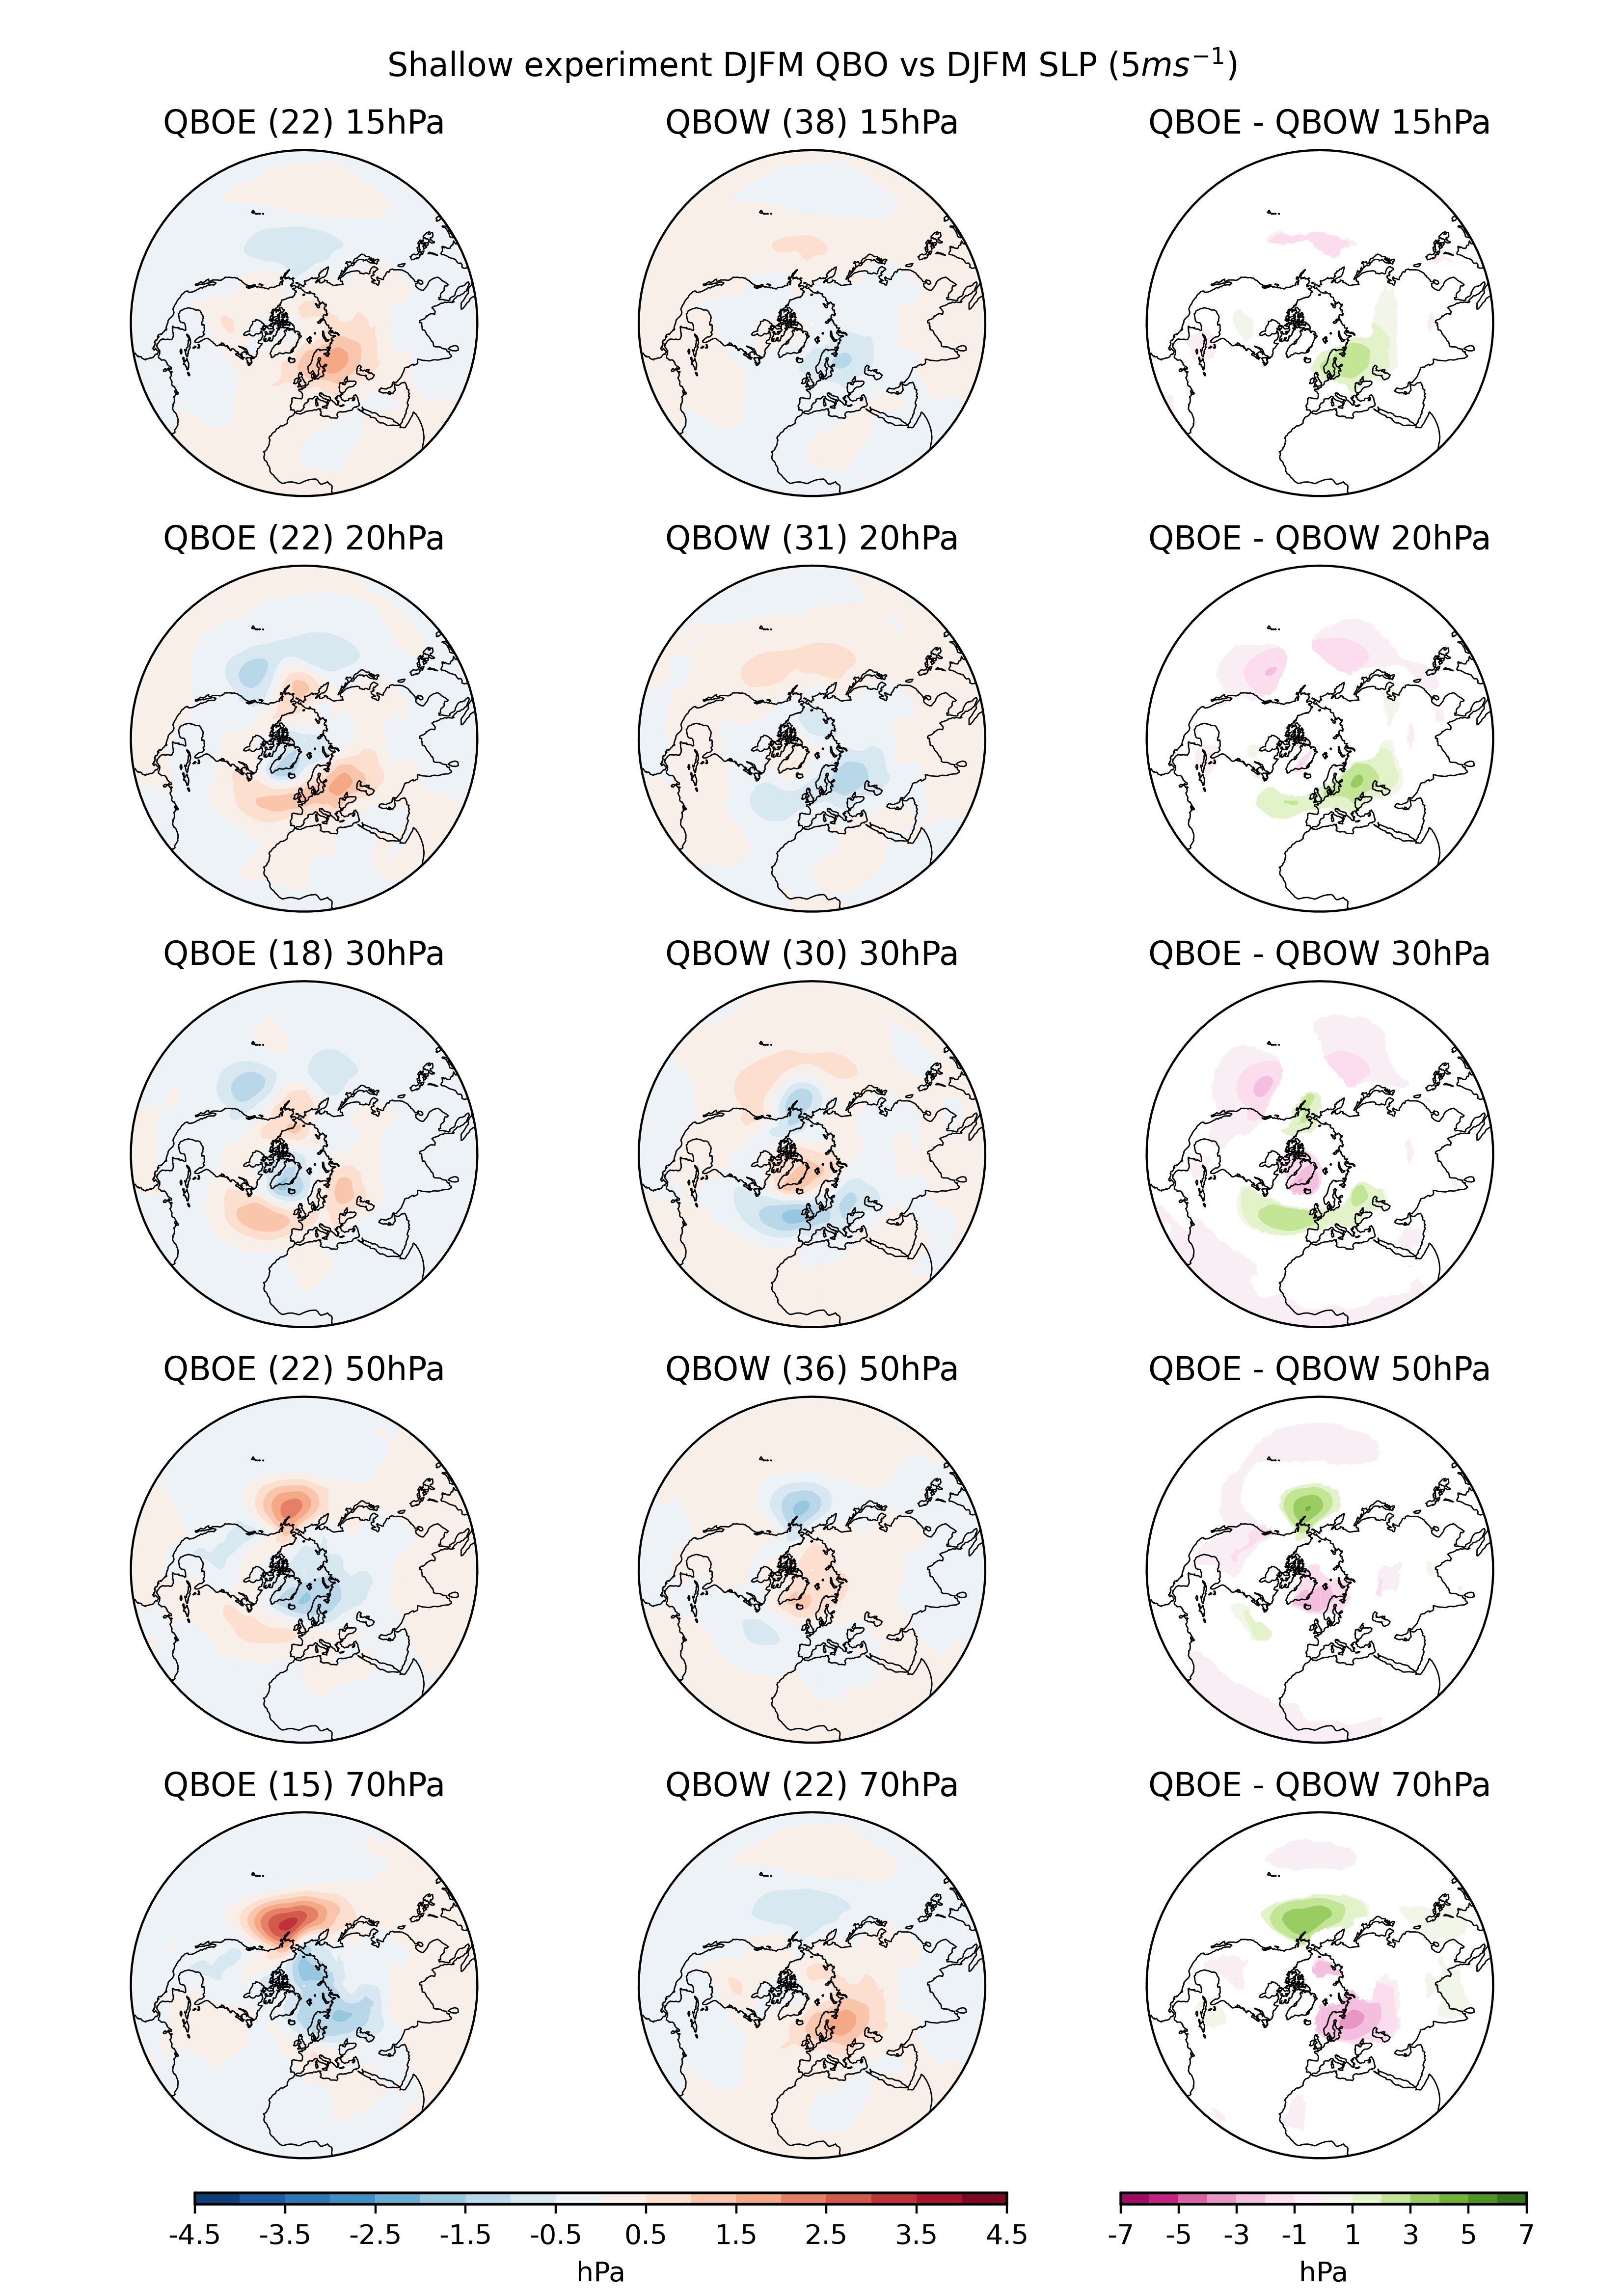
\includegraphics[width = \linewidth]{Figures/Figures-deepQBO/SLP_composites_QBO_phases_s_DJFMQBO_vs_DJFM_70hPa_5thresh.png}
\caption[Climatological seasonal cycle of equatorial ZMZW in QBO experiments]{Climatological seasonal cycle of ZMZW averaged between 5$^{\circ}$\,S--5$^{\circ}$\,N latitude from the deep (\textbf{a}) and shallow (\textbf{b}) QBO experiments. Panel \textbf{c} shows climatological differences between deep and shallow seasonal cycles. Black dots on (c) denote differences significant to the 95\% level under a 2-tailed student's t-test.}
\label{fig:experiment_SAOs}
\end{center}
\end{figure}





